\documentclass[]{book}
\usepackage{lmodern}
\usepackage{amssymb,amsmath}
\usepackage{ifxetex,ifluatex}
\usepackage{fixltx2e} % provides \textsubscript
\ifnum 0\ifxetex 1\fi\ifluatex 1\fi=0 % if pdftex
  \usepackage[T1]{fontenc}
  \usepackage[utf8]{inputenc}
\else % if luatex or xelatex
  \ifxetex
    \usepackage{mathspec}
  \else
    \usepackage{fontspec}
  \fi
  \defaultfontfeatures{Ligatures=TeX,Scale=MatchLowercase}
\fi
% use upquote if available, for straight quotes in verbatim environments
\IfFileExists{upquote.sty}{\usepackage{upquote}}{}
% use microtype if available
\IfFileExists{microtype.sty}{%
\usepackage{microtype}
\UseMicrotypeSet[protrusion]{basicmath} % disable protrusion for tt fonts
}{}
\usepackage[margin=1in]{geometry}
\usepackage{hyperref}
\hypersetup{unicode=true,
            pdftitle={Research Methods},
            pdfborder={0 0 0},
            breaklinks=true}
\urlstyle{same}  % don't use monospace font for urls
\usepackage{color}
\usepackage{fancyvrb}
\newcommand{\VerbBar}{|}
\newcommand{\VERB}{\Verb[commandchars=\\\{\}]}
\DefineVerbatimEnvironment{Highlighting}{Verbatim}{commandchars=\\\{\}}
% Add ',fontsize=\small' for more characters per line
\usepackage{framed}
\definecolor{shadecolor}{RGB}{248,248,248}
\newenvironment{Shaded}{\begin{snugshade}}{\end{snugshade}}
\newcommand{\KeywordTok}[1]{\textcolor[rgb]{0.13,0.29,0.53}{\textbf{#1}}}
\newcommand{\DataTypeTok}[1]{\textcolor[rgb]{0.13,0.29,0.53}{#1}}
\newcommand{\DecValTok}[1]{\textcolor[rgb]{0.00,0.00,0.81}{#1}}
\newcommand{\BaseNTok}[1]{\textcolor[rgb]{0.00,0.00,0.81}{#1}}
\newcommand{\FloatTok}[1]{\textcolor[rgb]{0.00,0.00,0.81}{#1}}
\newcommand{\ConstantTok}[1]{\textcolor[rgb]{0.00,0.00,0.00}{#1}}
\newcommand{\CharTok}[1]{\textcolor[rgb]{0.31,0.60,0.02}{#1}}
\newcommand{\SpecialCharTok}[1]{\textcolor[rgb]{0.00,0.00,0.00}{#1}}
\newcommand{\StringTok}[1]{\textcolor[rgb]{0.31,0.60,0.02}{#1}}
\newcommand{\VerbatimStringTok}[1]{\textcolor[rgb]{0.31,0.60,0.02}{#1}}
\newcommand{\SpecialStringTok}[1]{\textcolor[rgb]{0.31,0.60,0.02}{#1}}
\newcommand{\ImportTok}[1]{#1}
\newcommand{\CommentTok}[1]{\textcolor[rgb]{0.56,0.35,0.01}{\textit{#1}}}
\newcommand{\DocumentationTok}[1]{\textcolor[rgb]{0.56,0.35,0.01}{\textbf{\textit{#1}}}}
\newcommand{\AnnotationTok}[1]{\textcolor[rgb]{0.56,0.35,0.01}{\textbf{\textit{#1}}}}
\newcommand{\CommentVarTok}[1]{\textcolor[rgb]{0.56,0.35,0.01}{\textbf{\textit{#1}}}}
\newcommand{\OtherTok}[1]{\textcolor[rgb]{0.56,0.35,0.01}{#1}}
\newcommand{\FunctionTok}[1]{\textcolor[rgb]{0.00,0.00,0.00}{#1}}
\newcommand{\VariableTok}[1]{\textcolor[rgb]{0.00,0.00,0.00}{#1}}
\newcommand{\ControlFlowTok}[1]{\textcolor[rgb]{0.13,0.29,0.53}{\textbf{#1}}}
\newcommand{\OperatorTok}[1]{\textcolor[rgb]{0.81,0.36,0.00}{\textbf{#1}}}
\newcommand{\BuiltInTok}[1]{#1}
\newcommand{\ExtensionTok}[1]{#1}
\newcommand{\PreprocessorTok}[1]{\textcolor[rgb]{0.56,0.35,0.01}{\textit{#1}}}
\newcommand{\AttributeTok}[1]{\textcolor[rgb]{0.77,0.63,0.00}{#1}}
\newcommand{\RegionMarkerTok}[1]{#1}
\newcommand{\InformationTok}[1]{\textcolor[rgb]{0.56,0.35,0.01}{\textbf{\textit{#1}}}}
\newcommand{\WarningTok}[1]{\textcolor[rgb]{0.56,0.35,0.01}{\textbf{\textit{#1}}}}
\newcommand{\AlertTok}[1]{\textcolor[rgb]{0.94,0.16,0.16}{#1}}
\newcommand{\ErrorTok}[1]{\textcolor[rgb]{0.64,0.00,0.00}{\textbf{#1}}}
\newcommand{\NormalTok}[1]{#1}
\usepackage{longtable,booktabs}
\usepackage{graphicx,grffile}
\makeatletter
\def\maxwidth{\ifdim\Gin@nat@width>\linewidth\linewidth\else\Gin@nat@width\fi}
\def\maxheight{\ifdim\Gin@nat@height>\textheight\textheight\else\Gin@nat@height\fi}
\makeatother
% Scale images if necessary, so that they will not overflow the page
% margins by default, and it is still possible to overwrite the defaults
% using explicit options in \includegraphics[width, height, ...]{}
\setkeys{Gin}{width=\maxwidth,height=\maxheight,keepaspectratio}
\IfFileExists{parskip.sty}{%
\usepackage{parskip}
}{% else
\setlength{\parindent}{0pt}
\setlength{\parskip}{6pt plus 2pt minus 1pt}
}
\setlength{\emergencystretch}{3em}  % prevent overfull lines
\providecommand{\tightlist}{%
  \setlength{\itemsep}{0pt}\setlength{\parskip}{0pt}}
\setcounter{secnumdepth}{5}
% Redefines (sub)paragraphs to behave more like sections
\ifx\paragraph\undefined\else
\let\oldparagraph\paragraph
\renewcommand{\paragraph}[1]{\oldparagraph{#1}\mbox{}}
\fi
\ifx\subparagraph\undefined\else
\let\oldsubparagraph\subparagraph
\renewcommand{\subparagraph}[1]{\oldsubparagraph{#1}\mbox{}}
\fi

%%% Use protect on footnotes to avoid problems with footnotes in titles
\let\rmarkdownfootnote\footnote%
\def\footnote{\protect\rmarkdownfootnote}

%%% Change title format to be more compact
\usepackage{titling}

% Create subtitle command for use in maketitle
\newcommand{\subtitle}[1]{
  \posttitle{
    \begin{center}\large#1\end{center}
    }
}

\setlength{\droptitle}{-2em}

  \title{Research Methods}
    \pretitle{\vspace{\droptitle}\centering\huge}
  \posttitle{\par}
    \author{}
    \preauthor{}\postauthor{}
      \predate{\centering\large\emph}
  \postdate{\par}
    \date{2018-09-19}

\usepackage{booktabs}
\usepackage{amsthm}
\makeatletter
\def\thm@space@setup{%
  \thm@preskip=8pt plus 2pt minus 4pt
  \thm@postskip=\thm@preskip
}
\makeatother

\AtBeginDocument{\let\maketitle\relax} % supress header


\usepackage{fancyhdr}
\pagestyle{fancy}
% \fancyhead[CO,CE]{ZHAW LSFM}
\fancyfoot[CO,CE]{\textsc{zhaw lsfm}}
\fancyfoot[LE,RO]{\thepage}
\fancyfoot[RE,LO]{Modul \textit{ResearchMethods}}

\begin{document}
\maketitle

\newgeometry{tmargin=1.5cm,lmargin=2.5cm,rmargin=2.5cm,bmargin=0.5cm} %verbose

\begin{titlepage}
\begin{center}
  
{\small 
ZURICH UNIVERSITY OF APPLIED SCIENCES
\linebreak SCHOOL OF LIFE SCIENCES AND FACILITY MANAGEMENT
\linebreak INSTITUTE OF NATURAL RESOURCE SCIENCES
}

\end{center}
\vspace{1.5cm}
\begin{center}

{\Large Übungsunterlagen und Demoscript zum Modul \emph{Research Methods}}

\end{center}
 \vspace{1cm}

% \begin{figure}[htbp]
%   \centering
%   \includegraphics[width=1\textwidth]{Images/Reh-flucht-compilation3_small.png}
%   \label{titelbild} 
% \end{figure}

\begin{center}
\textbf{Herbstsemester 2017}

\textbf{Patrick Laube und Nils Ratnaweera}
% \linebreak
% Master of Life Sciences 2014
% \linebreak
% Submission date: 16. December 2016
\end{center} 

\vspace{1.0cm}

% \begin{table}[H]
%     \begin{tabular}{l}
%  %   \toprule
%     Supervisors: \\
%    % \midrule
%     Prof. Dr. Roland Felix Graf \\
%     Head of Research Group for Wildlife Management ZHAW\\
%     Life Sciences and Facility Management, Schloss, 8820 W{\"a}denswil \\
%      \\
% 		
% 		Dr. Patrick Laube \\
%     Head of GIScience research group ZHAW\\
%     Life Sciences and Facility Management, Gr{\"u}ental, 8820 W{\"a}denswil \\
%      \\
% 		
%     Dr. Claudio Signer \\
%     Research Fellow Research Group for Wildlife Management ZHAW\\
%     Life Sciences and Facility Management, Schloss, 8820 W{\"a}denswil \\
%      \\
%  %   \bottomrule
%     \end{tabular}%
%   \label{korrektoren}%
% \end{table}%

\newpage
\thispagestyle{empty}
\begin{minipage}{15cm}
\begin{flushleft}




\vspace{18cm}
{\large Impressum:}

\vspace{0.5cm}

% \textbf{Citation:} 
Laube, P. \& Ratnawera N. (2017): Übungsunterlagen für das Modul Research Methods im Master of Science in Umwelt und Natürliche Ressourcen. IUNR, Zürcher Hochschule der Angewandten Wissenschaften (ZHAW), W{\"a}denswil.

\end{flushleft}
\end{minipage}

\end{titlepage}
\restoregeometry

{
\setcounter{tocdepth}{1}
\tableofcontents
}
\chapter{Einleitung}\label{einleitung}

Das Modul „Research Methods`` vermittelt vertiefte Methodenkompetenzen
für praxisorientiertes und angewandtes wissenschaftliches Arbeiten im
Fachbereich „Umwelt und Natürliche Ressourcen`` auf MSc-Niveau. Die
Studierenden erarbeiten sich vertiefte Methodenkompetenzen für die
analytische Betrachtung der Zusammenhänge im Gesamtsystem „Umwelt und
Natürliche Ressourcen``. Die Studierenden erlernen die methodischen
Kompetenzen, auf denen die nachfolgenden Module im MSc Programm UNR
aufbauen. Das Modul vermittelt einerseits allgemeine,
fächerübergreifende methodische Kompetenzen (z.B. Wissenschaftstheorie,
computer-gestützte Datenverar-beitung und Statistik).

Auf dieser Plattform (RStudio Connect) werden die Unterlagen für die
R-Übungsteile bereitgestellt. Es werden sukzessive sowohl Demo-Files,
Aufgabenstellungen und Lösungen veröffentlicht.

\chapter{Statistik 1 (30.10.17)}\label{statistik-1-30.10.17}

In Statistik 1 lernen die Studierenden, was (Inferenz-) Statistik im
Kern leistet und warum sie für wissenschaftliche Erkenntnis (in den
meisten Disziplinen) unentbehrlich ist. Nach einer Wiederholung der
Rolle von Hypothesen wird erläutert, wie Hypothesentests in der
frequentist-Statistik umgesetzt werden, einschliesslich p-Werten und
Signifikanz-Levels. Die praktische Statistik beginnt mit den beiden
einfachsten Fällen, dem Chi-Quadrat-Test für die Assoziation zwischen
zwei kategorialen Variablen und dem t-Test auf Unterschiede in
Mittelwerten zwischen zwei Gruppen. Dann geht es um die Voraussetzungen
parametrischer (und nicht-parametrischer) Tests und Optionen, wenn diese
verletzt sind. Abschliessend gibt es einen ersten Einstieg in die
Varianzanalyse (ANOVA).

\section{Demo: Stastische Tests}\label{demo-stastische-tests}

\href{13_Statistik1/RFiles/Demo_Tests.R}{Demoscript als Download}

\subsection{Assoziationstests}\label{assoziationstests}

\begin{Shaded}
\begin{Highlighting}[]
\KeywordTok{library}\NormalTok{(car)}
\KeywordTok{library}\NormalTok{(tidyverse)}

\KeywordTok{library}\NormalTok{(ggfortify)}

\NormalTok{select <-}\StringTok{ }\NormalTok{dplyr}\OperatorTok{::}\NormalTok{select}
\end{Highlighting}
\end{Shaded}

\begin{Shaded}
\begin{Highlighting}[]

\CommentTok{# Chi-Quadrat-Test}

\CommentTok{# Ermitteln des kritischen Wertes für 95 perzentile und 1 FG}
\KeywordTok{qchisq}\NormalTok{(}\FloatTok{0.95}\NormalTok{,}\DecValTok{1}\NormalTok{)}
\NormalTok{## [1] 3.841459}
\end{Highlighting}
\end{Shaded}

\begin{Shaded}
\begin{Highlighting}[]

\CommentTok{# Datensatz von Folie 28: Test auf Assoziation zwischen zwei kategorialen Variablen}
\CommentTok{# Frage: Wie hängen zwei Eigenschaften des gleichen Objektes zusammen?}

\NormalTok{count <-}\StringTok{ }\KeywordTok{matrix}\NormalTok{(}\KeywordTok{c}\NormalTok{(}\DecValTok{38}\NormalTok{,}\DecValTok{14}\NormalTok{,}\DecValTok{11}\NormalTok{,}\DecValTok{51}\NormalTok{),}\DataTypeTok{nrow=}\DecValTok{2}\NormalTok{)}

\NormalTok{count}
\NormalTok{##      [,1] [,2]}
\NormalTok{## [1,]   38   11}
\NormalTok{## [2,]   14   51}

\KeywordTok{dimnames}\NormalTok{(count) <-}\StringTok{ }\KeywordTok{list}\NormalTok{(}\KeywordTok{c}\NormalTok{(}\StringTok{"helle_haare"}\NormalTok{,}\StringTok{"hunkle_haare"}\NormalTok{),}\KeywordTok{c}\NormalTok{(}\StringTok{"blaue_augen"}\NormalTok{,}\StringTok{"braune_augen"}\NormalTok{))}

\NormalTok{count}
\NormalTok{##              blaue_augen braune_augen}
\NormalTok{## helle_haare           38           11}
\NormalTok{## hunkle_haare          14           51}

\KeywordTok{chisq.test}\NormalTok{(count)}
\NormalTok{## }
\NormalTok{##  Pearson's Chi-squared test with Yates' continuity correction}
\NormalTok{## }
\NormalTok{## data:  count}
\NormalTok{## X-squared = 33.112, df = 1, p-value = 8.7e-09}

\KeywordTok{chisq.test}\NormalTok{(count,}\DataTypeTok{correct =}\NormalTok{ F)}
\NormalTok{## }
\NormalTok{##  Pearson's Chi-squared test}
\NormalTok{## }
\NormalTok{## data:  count}
\NormalTok{## X-squared = 35.334, df = 1, p-value = 2.778e-09}

\KeywordTok{fisher.test}\NormalTok{(count)}
\NormalTok{## }
\NormalTok{##  Fisher's Exact Test for Count Data}
\NormalTok{## }
\NormalTok{## data:  count}
\NormalTok{## p-value = 2.099e-09}
\NormalTok{## alternative hypothesis: true odds ratio is not equal to 1}
\NormalTok{## 95 percent confidence interval:}
\NormalTok{##   4.746351 34.118920}
\NormalTok{## sample estimates:}
\NormalTok{## odds ratio }
\NormalTok{##   12.22697}
\end{Highlighting}
\end{Shaded}

\subsection{t-Test}\label{t-test}

\begin{Shaded}
\begin{Highlighting}[]

\CommentTok{# Datensatz "Blumen" erstellen für t-Test}

\NormalTok{blume <-}\KeywordTok{data.frame}\NormalTok{(}
  \DataTypeTok{sorte_a =} \KeywordTok{c}\NormalTok{(}\DecValTok{20}\NormalTok{,}\DecValTok{19}\NormalTok{,}\DecValTok{25}\NormalTok{,}\DecValTok{10}\NormalTok{,}\DecValTok{8}\NormalTok{,}\DecValTok{15}\NormalTok{,}\DecValTok{13}\NormalTok{,}\DecValTok{18}\NormalTok{,}\DecValTok{11}\NormalTok{,}\DecValTok{14}\NormalTok{),}
  \DataTypeTok{sorte_b =} \KeywordTok{c}\NormalTok{(}\DecValTok{12}\NormalTok{,}\DecValTok{15}\NormalTok{,}\DecValTok{16}\NormalTok{,}\DecValTok{7}\NormalTok{,}\DecValTok{8}\NormalTok{,}\DecValTok{10}\NormalTok{,}\DecValTok{12}\NormalTok{,}\DecValTok{11}\NormalTok{,}\DecValTok{13}\NormalTok{,}\DecValTok{10}\NormalTok{)}
\NormalTok{  )}

\NormalTok{blume}
\NormalTok{##    sorte_a sorte_b}
\NormalTok{## 1       20      12}
\NormalTok{## 2       19      15}
\NormalTok{## 3       25      16}
\NormalTok{## 4       10       7}
\NormalTok{## 5        8       8}
\NormalTok{## 6       15      10}
\NormalTok{## 7       13      12}
\NormalTok{## 8       18      11}
\NormalTok{## 9       11      13}
\NormalTok{## 10      14      10}
\KeywordTok{summary}\NormalTok{(blume)}
\NormalTok{##     sorte_a         sorte_b     }
\NormalTok{##  Min.   : 8.00   Min.   : 7.00  }
\NormalTok{##  1st Qu.:11.50   1st Qu.:10.00  }
\NormalTok{##  Median :14.50   Median :11.50  }
\NormalTok{##  Mean   :15.30   Mean   :11.40  }
\NormalTok{##  3rd Qu.:18.75   3rd Qu.:12.75  }
\NormalTok{##  Max.   :25.00   Max.   :16.00}
\end{Highlighting}
\end{Shaded}

\subsubsection{\texorpdfstring{Tests mit einer \emph{breiten} (wide)
Tabelle}{Tests mit einer breiten (wide) Tabelle}}\label{tests-mit-einer-breiten-wide-tabelle}

\begin{Shaded}
\begin{Highlighting}[]



\KeywordTok{boxplot}\NormalTok{(blume}\OperatorTok{$}\NormalTok{sorte_a,blume}\OperatorTok{$}\NormalTok{sorte_b)}
\end{Highlighting}
\end{Shaded}

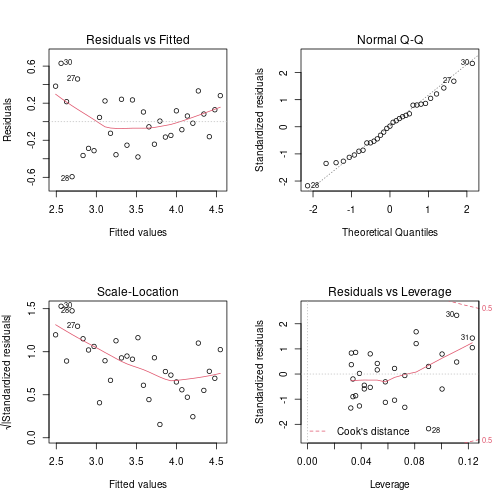
\includegraphics{ResearchMethods_files/figure-latex/unnamed-chunk-10-1.pdf}

\begin{Shaded}
\begin{Highlighting}[]

\KeywordTok{hist}\NormalTok{(blume}\OperatorTok{$}\NormalTok{sorte_a)}
\end{Highlighting}
\end{Shaded}

\includegraphics{ResearchMethods_files/figure-latex/unnamed-chunk-10-2.pdf}

\begin{Shaded}
\begin{Highlighting}[]

\KeywordTok{hist}\NormalTok{(blume}\OperatorTok{$}\NormalTok{sorte_b)}
\end{Highlighting}
\end{Shaded}

\includegraphics{ResearchMethods_files/figure-latex/unnamed-chunk-10-3.pdf}

\begin{Shaded}
\begin{Highlighting}[]

\KeywordTok{t.test}\NormalTok{(blume}\OperatorTok{$}\NormalTok{sorte_a,blume}\OperatorTok{$}\NormalTok{sorte_b) }\CommentTok{#zweiseitig}
\NormalTok{## }
\NormalTok{##  Welch Two Sample t-test}
\NormalTok{## }
\NormalTok{## data:  blume$sorte_a and blume$sorte_b}
\NormalTok{## t = 2.0797, df = 13.907, p-value = 0.05654}
\NormalTok{## alternative hypothesis: true difference in means is not equal to 0}
\NormalTok{## 95 percent confidence interval:}
\NormalTok{##  -0.1245926  7.9245926}
\NormalTok{## sample estimates:}
\NormalTok{## mean of x mean of y }
\NormalTok{##      15.3      11.4}
\KeywordTok{t.test}\NormalTok{(blume}\OperatorTok{$}\NormalTok{sorte_a,blume}\OperatorTok{$}\NormalTok{sorte_b, }\DataTypeTok{alternative=}\StringTok{"greater"}\NormalTok{) }\CommentTok{#einseitig}
\NormalTok{## }
\NormalTok{##  Welch Two Sample t-test}
\NormalTok{## }
\NormalTok{## data:  blume$sorte_a and blume$sorte_b}
\NormalTok{## t = 2.0797, df = 13.907, p-value = 0.02827}
\NormalTok{## alternative hypothesis: true difference in means is greater than 0}
\NormalTok{## 95 percent confidence interval:}
\NormalTok{##  0.5954947       Inf}
\NormalTok{## sample estimates:}
\NormalTok{## mean of x mean of y }
\NormalTok{##      15.3      11.4}
\KeywordTok{t.test}\NormalTok{(blume}\OperatorTok{$}\NormalTok{sorte_a,blume}\OperatorTok{$}\NormalTok{sorte_b, }\DataTypeTok{alternative=}\StringTok{"less"}\NormalTok{) }\CommentTok{#einseitig}
\NormalTok{## }
\NormalTok{##  Welch Two Sample t-test}
\NormalTok{## }
\NormalTok{## data:  blume$sorte_a and blume$sorte_b}
\NormalTok{## t = 2.0797, df = 13.907, p-value = 0.9717}
\NormalTok{## alternative hypothesis: true difference in means is less than 0}
\NormalTok{## 95 percent confidence interval:}
\NormalTok{##      -Inf 7.204505}
\NormalTok{## sample estimates:}
\NormalTok{## mean of x mean of y }
\NormalTok{##      15.3      11.4}
\KeywordTok{t.test}\NormalTok{(blume}\OperatorTok{$}\NormalTok{sorte_a,blume}\OperatorTok{$}\NormalTok{sorte_b, }\DataTypeTok{var.equal=}\NormalTok{T) }\CommentTok{#Varianzen gleich, klassischer t-Test}
\NormalTok{## }
\NormalTok{##  Two Sample t-test}
\NormalTok{## }
\NormalTok{## data:  blume$sorte_a and blume$sorte_b}
\NormalTok{## t = 2.0797, df = 18, p-value = 0.05212}
\NormalTok{## alternative hypothesis: true difference in means is not equal to 0}
\NormalTok{## 95 percent confidence interval:}
\NormalTok{##  -0.03981237  7.83981237}
\NormalTok{## sample estimates:}
\NormalTok{## mean of x mean of y }
\NormalTok{##      15.3      11.4}
\KeywordTok{t.test}\NormalTok{(blume}\OperatorTok{$}\NormalTok{sorte_a,blume}\OperatorTok{$}\NormalTok{sorte_b, }\DataTypeTok{var.equal=}\NormalTok{F) }\CommentTok{#Varianzen ungleich, Welch's t-Test, ist auch default}
\NormalTok{## }
\NormalTok{##  Welch Two Sample t-test}
\NormalTok{## }
\NormalTok{## data:  blume$sorte_a and blume$sorte_b}
\NormalTok{## t = 2.0797, df = 13.907, p-value = 0.05654}
\NormalTok{## alternative hypothesis: true difference in means is not equal to 0}
\NormalTok{## 95 percent confidence interval:}
\NormalTok{##  -0.1245926  7.9245926}
\NormalTok{## sample estimates:}
\NormalTok{## mean of x mean of y }
\NormalTok{##      15.3      11.4}
\KeywordTok{t.test}\NormalTok{(blume}\OperatorTok{$}\NormalTok{sorte_a,blume}\OperatorTok{$}\NormalTok{sorte_b, }\DataTypeTok{paired=}\NormalTok{T) }\CommentTok{#gepaarter t-Test }
\NormalTok{## }
\NormalTok{##  Paired t-test}
\NormalTok{## }
\NormalTok{## data:  blume$sorte_a and blume$sorte_b}
\NormalTok{## t = 3.4821, df = 9, p-value = 0.006916}
\NormalTok{## alternative hypothesis: true difference in means is not equal to 0}
\NormalTok{## 95 percent confidence interval:}
\NormalTok{##  1.366339 6.433661}
\NormalTok{## sample estimates:}
\NormalTok{## mean of the differences }
\NormalTok{##                     3.9}
\KeywordTok{t.test}\NormalTok{(blume}\OperatorTok{$}\NormalTok{sorte_a,blume}\OperatorTok{$}\NormalTok{sorte_b, }\DataTypeTok{paired=}\NormalTok{T,}\DataTypeTok{alternative=}\StringTok{"greater"}\NormalTok{) }\CommentTok{#gepaarter t-Test }
\NormalTok{## }
\NormalTok{##  Paired t-test}
\NormalTok{## }
\NormalTok{## data:  blume$sorte_a and blume$sorte_b}
\NormalTok{## t = 3.4821, df = 9, p-value = 0.003458}
\NormalTok{## alternative hypothesis: true difference in means is greater than 0}
\NormalTok{## 95 percent confidence interval:}
\NormalTok{##  1.846877      Inf}
\NormalTok{## sample estimates:}
\NormalTok{## mean of the differences }
\NormalTok{##                     3.9}

\KeywordTok{shapiro.test}\NormalTok{(blume}\OperatorTok{$}\NormalTok{sorte_b)}
\NormalTok{## }
\NormalTok{##  Shapiro-Wilk normality test}
\NormalTok{## }
\NormalTok{## data:  blume$sorte_b}
\NormalTok{## W = 0.97341, p-value = 0.9206}

\KeywordTok{wilcox.test}\NormalTok{(blume}\OperatorTok{$}\NormalTok{sorte_a,blume}\OperatorTok{$}\NormalTok{sorte_b)}
\NormalTok{## Warning in wilcox.test.default(blume$sorte_a, blume$sorte_b): cannot}
\NormalTok{## compute exact p-value with ties}
\NormalTok{## }
\NormalTok{##  Wilcoxon rank sum test with continuity correction}
\NormalTok{## }
\NormalTok{## data:  blume$sorte_a and blume$sorte_b}
\NormalTok{## W = 73, p-value = 0.08789}
\NormalTok{## alternative hypothesis: true location shift is not equal to 0}
\end{Highlighting}
\end{Shaded}

\subsubsection{\texorpdfstring{Tests mit einer \emph{langen} (long)
Tabelle}{Tests mit einer langen (long) Tabelle}}\label{tests-mit-einer-langen-long-tabelle}

\begin{Shaded}
\begin{Highlighting}[]
\CommentTok{# T-Tests mit einer langen (long) Tabelle}

\CommentTok{# breit zu long mit tidyr::gather}

\NormalTok{blume_long <-}\StringTok{ }\KeywordTok{gather}\NormalTok{(blume,sorte,groesse)}

\CommentTok{# Für eine Long table können wir auch gut ggplot verwenden}

\KeywordTok{ggplot}\NormalTok{(blume_long, }\KeywordTok{aes}\NormalTok{(sorte, groesse)) }\OperatorTok{+}
\StringTok{  }\KeywordTok{geom_boxplot}\NormalTok{()}
\end{Highlighting}
\end{Shaded}

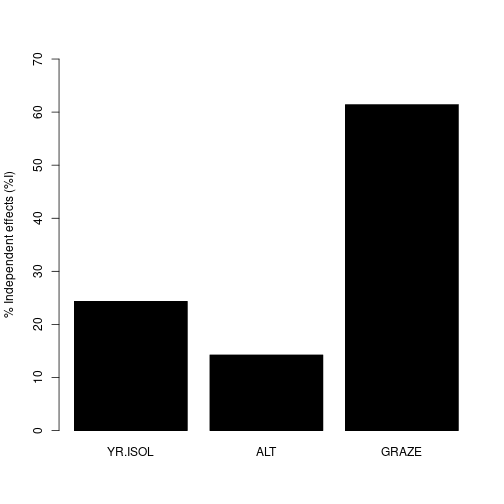
\includegraphics{ResearchMethods_files/figure-latex/unnamed-chunk-11-1.pdf}

\begin{Shaded}
\begin{Highlighting}[]

\KeywordTok{ggplot}\NormalTok{(blume_long, }\KeywordTok{aes}\NormalTok{(groesse)) }\OperatorTok{+}
\StringTok{  }\KeywordTok{geom_histogram}\NormalTok{(}\DataTypeTok{binwidth =} \DecValTok{1}\NormalTok{, }\DataTypeTok{colour =} \StringTok{"white"}\NormalTok{)}
\end{Highlighting}
\end{Shaded}

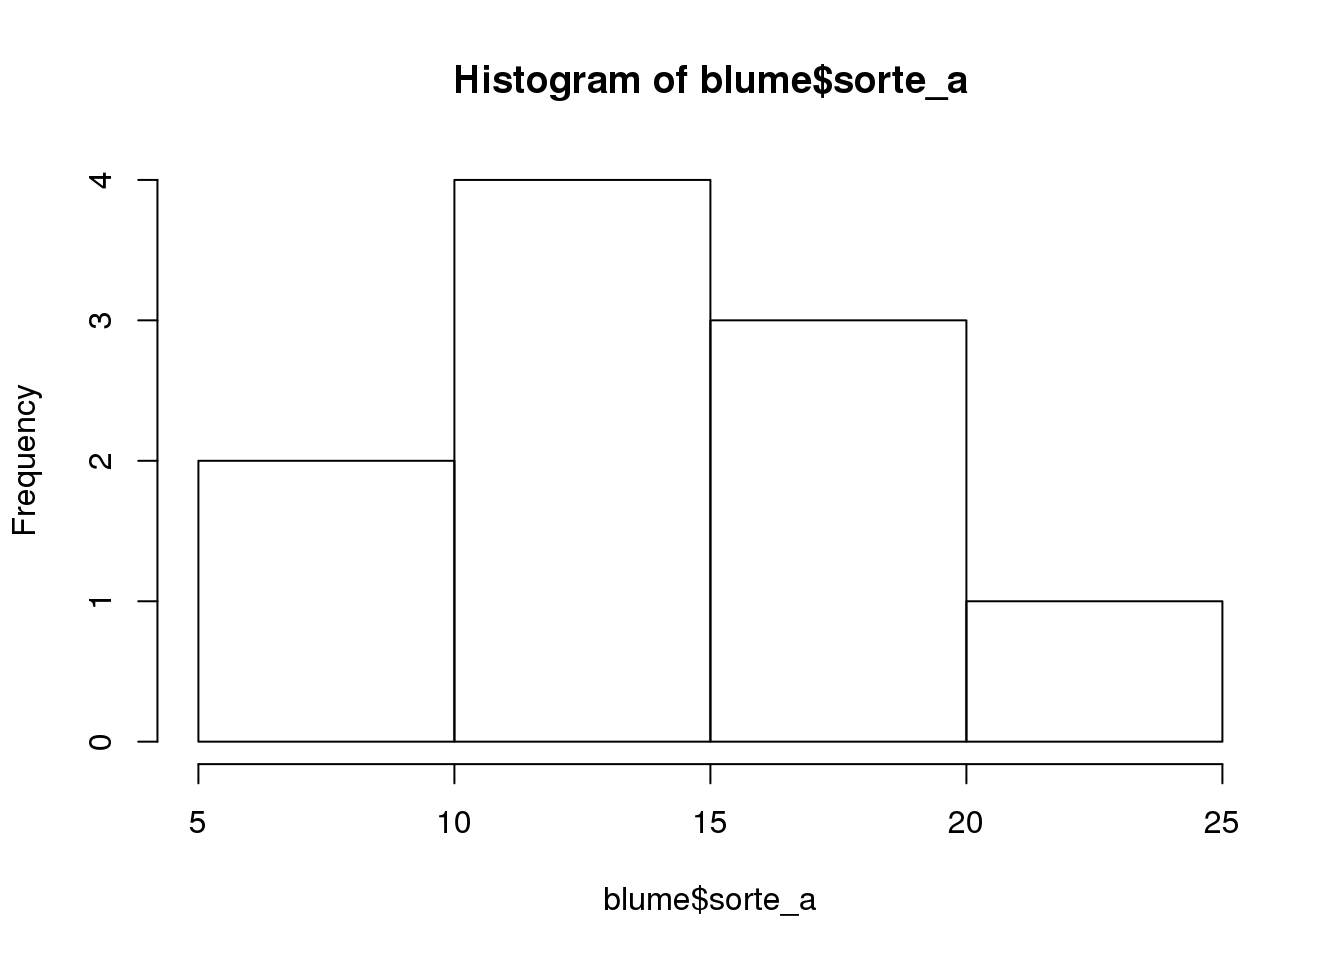
\includegraphics{ResearchMethods_files/figure-latex/unnamed-chunk-11-2.pdf}

\begin{Shaded}
\begin{Highlighting}[]

\KeywordTok{ggplot}\NormalTok{(blume_long, }\KeywordTok{aes}\NormalTok{(groesse)) }\OperatorTok{+}
\StringTok{  }\KeywordTok{geom_histogram}\NormalTok{(}\DataTypeTok{binwidth =} \DecValTok{2}\NormalTok{, }\DataTypeTok{colour =} \StringTok{"white"}\NormalTok{)}\OperatorTok{+}
\StringTok{  }\KeywordTok{facet_grid}\NormalTok{(sorte}\OperatorTok{~}\NormalTok{.)}
\end{Highlighting}
\end{Shaded}

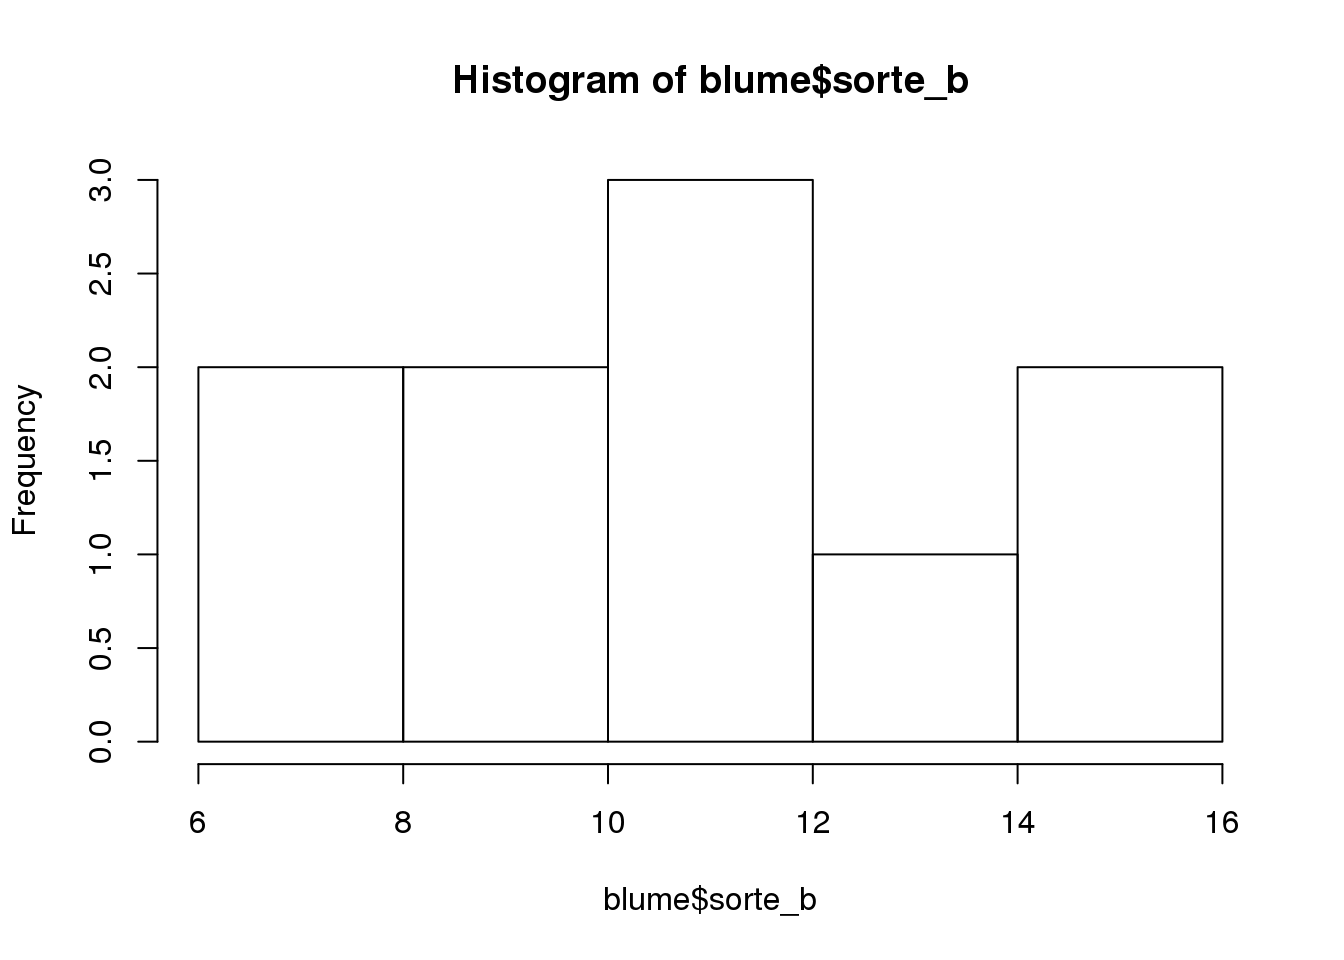
\includegraphics{ResearchMethods_files/figure-latex/unnamed-chunk-11-3.pdf}

\begin{Shaded}
\begin{Highlighting}[]

\KeywordTok{ggplot}\NormalTok{(blume_long, }\KeywordTok{aes}\NormalTok{(groesse, }\DataTypeTok{fill =}\NormalTok{ sorte)) }\OperatorTok{+}
\StringTok{  }\KeywordTok{geom_density}\NormalTok{(}\DataTypeTok{alpha =} \FloatTok{0.5}\NormalTok{)}
\end{Highlighting}
\end{Shaded}

\includegraphics{ResearchMethods_files/figure-latex/unnamed-chunk-11-4.pdf}

\begin{Shaded}
\begin{Highlighting}[]




\KeywordTok{t.test}\NormalTok{(groesse}\OperatorTok{~}\NormalTok{sorte, blume_long)}
\NormalTok{## }
\NormalTok{##  Welch Two Sample t-test}
\NormalTok{## }
\NormalTok{## data:  groesse by sorte}
\NormalTok{## t = 2.0797, df = 13.907, p-value = 0.05654}
\NormalTok{## alternative hypothesis: true difference in means is not equal to 0}
\NormalTok{## 95 percent confidence interval:}
\NormalTok{##  -0.1245926  7.9245926}
\NormalTok{## sample estimates:}
\NormalTok{## mean in group sorte_a mean in group sorte_b }
\NormalTok{##                  15.3                  11.4}

\CommentTok{# Optionen "alternative" und "var.equal" werden angepasst analog der "wide" table}
\end{Highlighting}
\end{Shaded}

\subsection{Randomisierung}\label{randomisierung}

Datensatz: \href{13_Statistik1/data/beetle.csv}{beetle.csv}

\begin{Shaded}
\begin{Highlighting}[]
\CommentTok{# Randomisierung}

\NormalTok{beetles <-}\StringTok{ }\KeywordTok{read_delim}\NormalTok{(}\StringTok{"13_Statistik1/data/beetle.csv"}\NormalTok{, }\StringTok{","}\NormalTok{)}
\NormalTok{## Parsed with column specification:}
\NormalTok{## cols(}
\NormalTok{##   SIZE = col_character(),}
\NormalTok{##   BEETLES = col_integer()}
\NormalTok{## )}


\KeywordTok{ggplot}\NormalTok{(beetles, }\KeywordTok{aes}\NormalTok{(SIZE, BEETLES)) }\OperatorTok{+}
\StringTok{  }\KeywordTok{geom_boxplot}\NormalTok{()}
\end{Highlighting}
\end{Shaded}

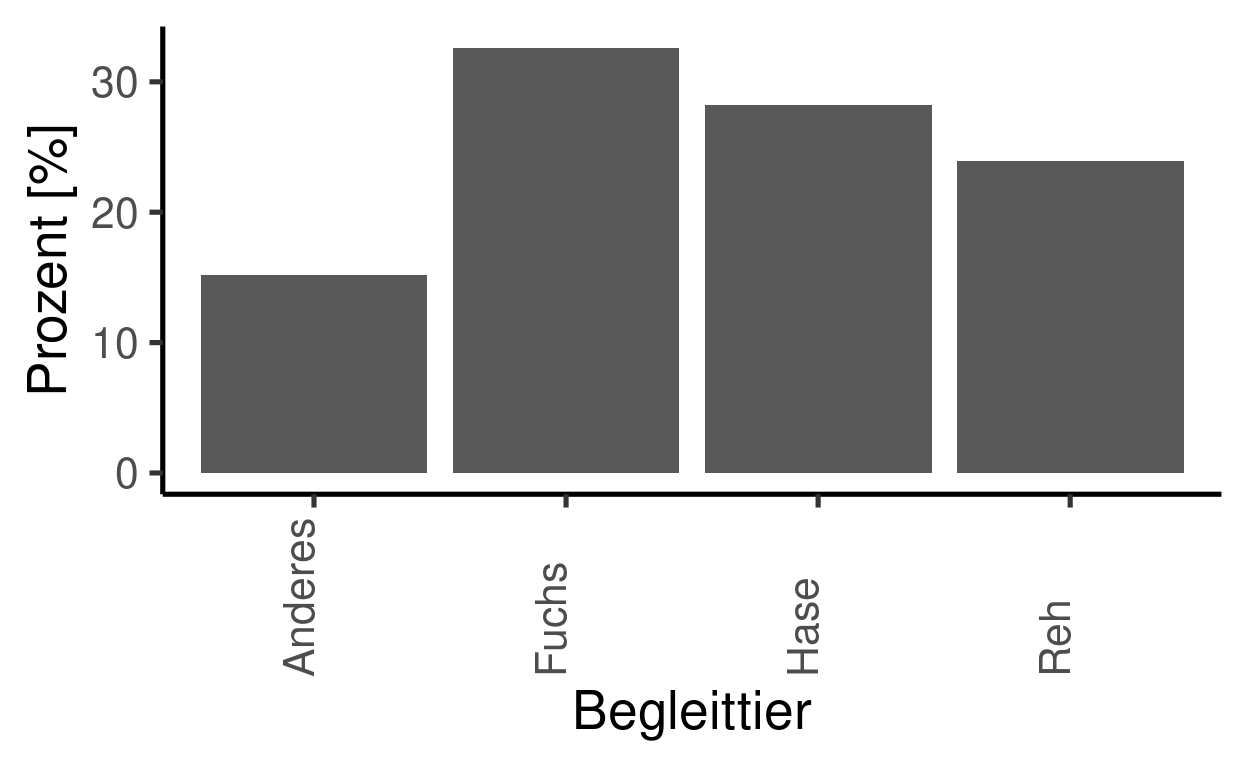
\includegraphics{ResearchMethods_files/figure-latex/unnamed-chunk-12-1.pdf}

\begin{Shaded}
\begin{Highlighting}[]


\KeywordTok{ggplot}\NormalTok{(beetles, }\KeywordTok{aes}\NormalTok{(SIZE, }\KeywordTok{sqrt}\NormalTok{(BEETLES))) }\OperatorTok{+}
\StringTok{  }\KeywordTok{geom_boxplot}\NormalTok{()}
\end{Highlighting}
\end{Shaded}

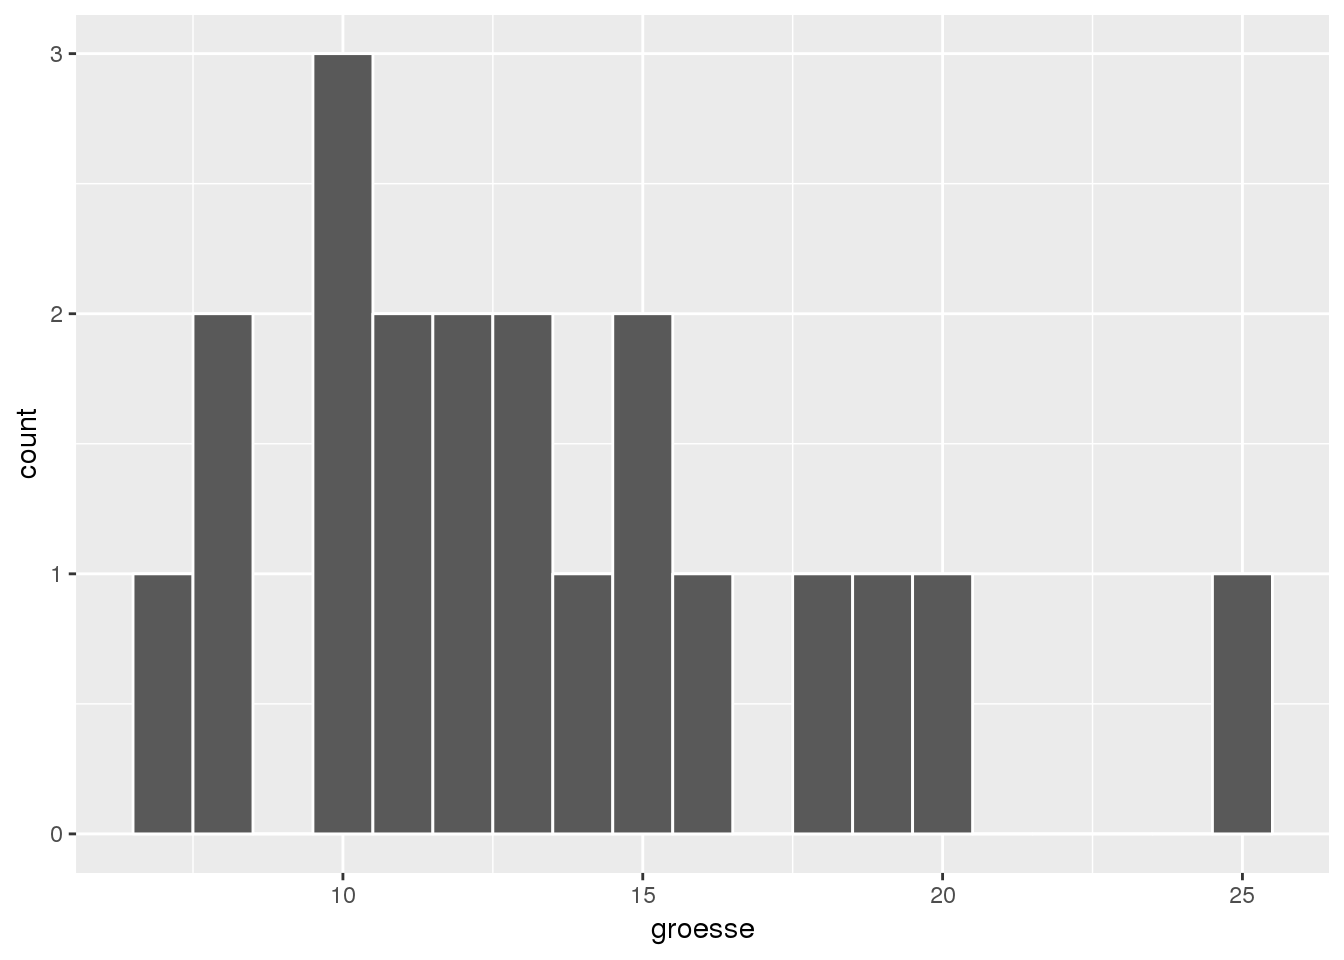
\includegraphics{ResearchMethods_files/figure-latex/unnamed-chunk-12-2.pdf}

\begin{Shaded}
\begin{Highlighting}[]


\KeywordTok{ggplot}\NormalTok{(beetles, }\KeywordTok{aes}\NormalTok{(SIZE, BEETLES)) }\OperatorTok{+}
\StringTok{  }\KeywordTok{geom_boxplot}\NormalTok{() }\OperatorTok{+}
\StringTok{  }\KeywordTok{scale_y_sqrt}\NormalTok{()}
\end{Highlighting}
\end{Shaded}

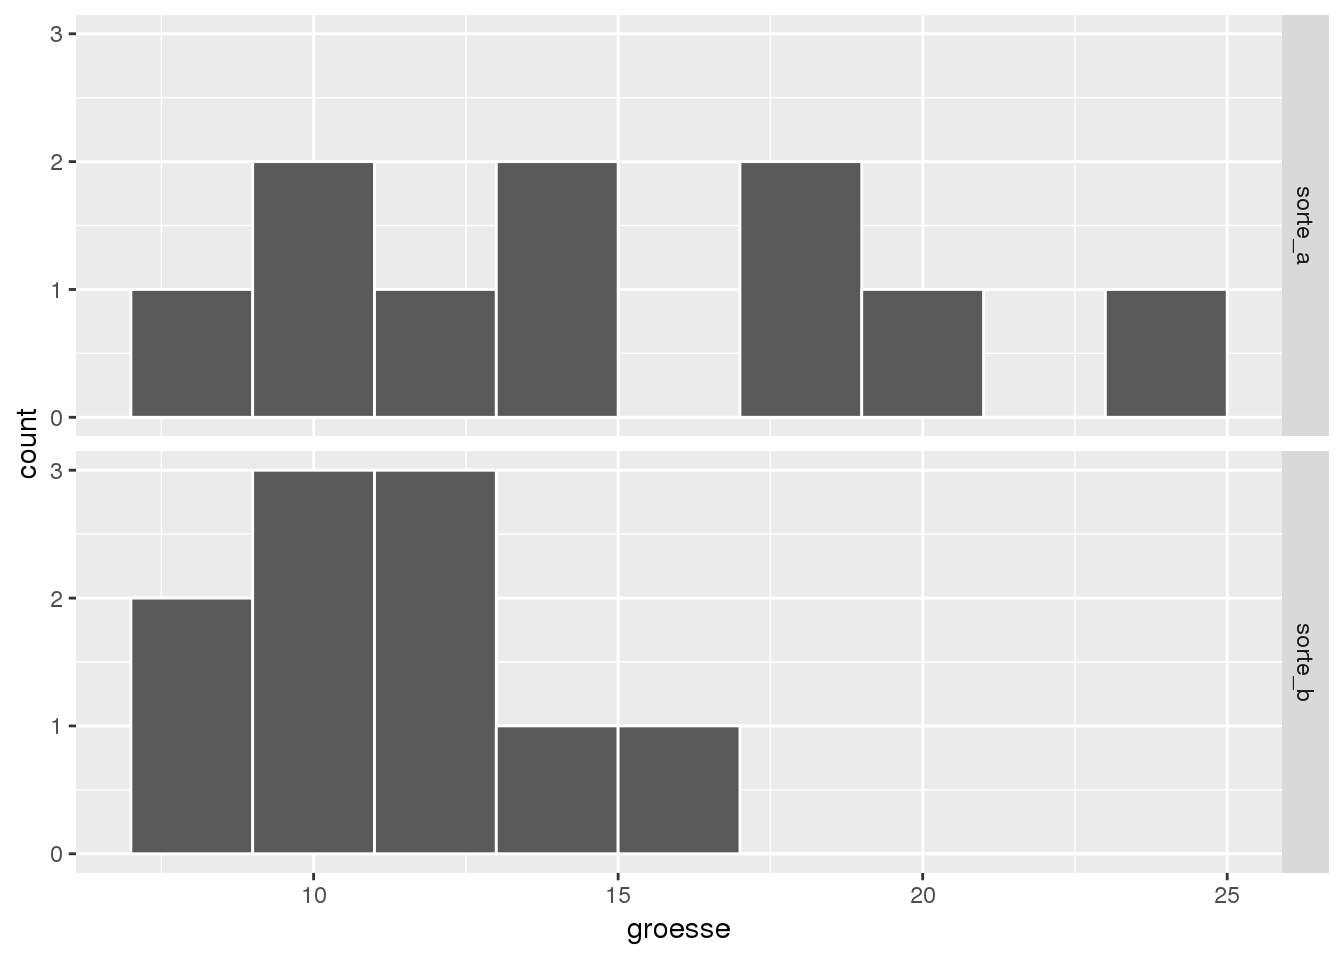
\includegraphics{ResearchMethods_files/figure-latex/unnamed-chunk-12-3.pdf}

\begin{Shaded}
\begin{Highlighting}[]


\CommentTok{# extract specific inidies from t-test}
\NormalTok{stat <-}\StringTok{ }\ControlFlowTok{function}\NormalTok{(data, indices) \{}
\NormalTok{  t.test <-}\StringTok{ }\KeywordTok{t.test}\NormalTok{(BEETLES}\OperatorTok{~}\NormalTok{SIZE, data)}\OperatorTok{$}\StringTok{"stat"}
\NormalTok{  t.test}
\NormalTok{\}}


\CommentTok{# Random generator auf der Basis eines Datensatzes}
\NormalTok{rand.gen <-}\StringTok{ }\ControlFlowTok{function}\NormalTok{(data,mle) \{}
\NormalTok{  out <-}\StringTok{ }\NormalTok{data}
\NormalTok{  out}\OperatorTok{$}\NormalTok{SIZE <-}\StringTok{ }\KeywordTok{sample}\NormalTok{(out}\OperatorTok{$}\NormalTok{SIZE, }\DataTypeTok{replace=}\NormalTok{F)}
\NormalTok{  out}
\NormalTok{\}}


\KeywordTok{library}\NormalTok{(boot)}
\NormalTok{## }
\NormalTok{## Attaching package: 'boot'}
\NormalTok{## The following object is masked from 'package:car':}
\NormalTok{## }
\NormalTok{##     logit}

\CommentTok{# boot(): bootstrap resampling}

\NormalTok{beetles.boot <-}\StringTok{ }\KeywordTok{boot}\NormalTok{(}\DataTypeTok{data =}\NormalTok{ beetles,}
                     \DataTypeTok{statistic =}\NormalTok{ stat, }
                     \DataTypeTok{R=}\DecValTok{5000}\NormalTok{, }
                     \DataTypeTok{sim=}\StringTok{"parametric"}\NormalTok{, }
                     \DataTypeTok{ran.gen=}\NormalTok{rand.gen)}


\KeywordTok{print}\NormalTok{(beetles.boot)}
\NormalTok{## }
\NormalTok{## PARAMETRIC BOOTSTRAP}
\NormalTok{## }
\NormalTok{## }
\NormalTok{## Call:}
\NormalTok{## boot(data = beetles, statistic = stat, R = 5000, sim = "parametric", }
\NormalTok{##     ran.gen = rand.gen)}
\NormalTok{## }
\NormalTok{## }
\NormalTok{## Bootstrap Statistics :}
\NormalTok{##     original    bias    std. error}
\NormalTok{## t1* 2.190697 -2.216792    1.016413}



\KeywordTok{plot}\NormalTok{(beetles.boot)}
\end{Highlighting}
\end{Shaded}

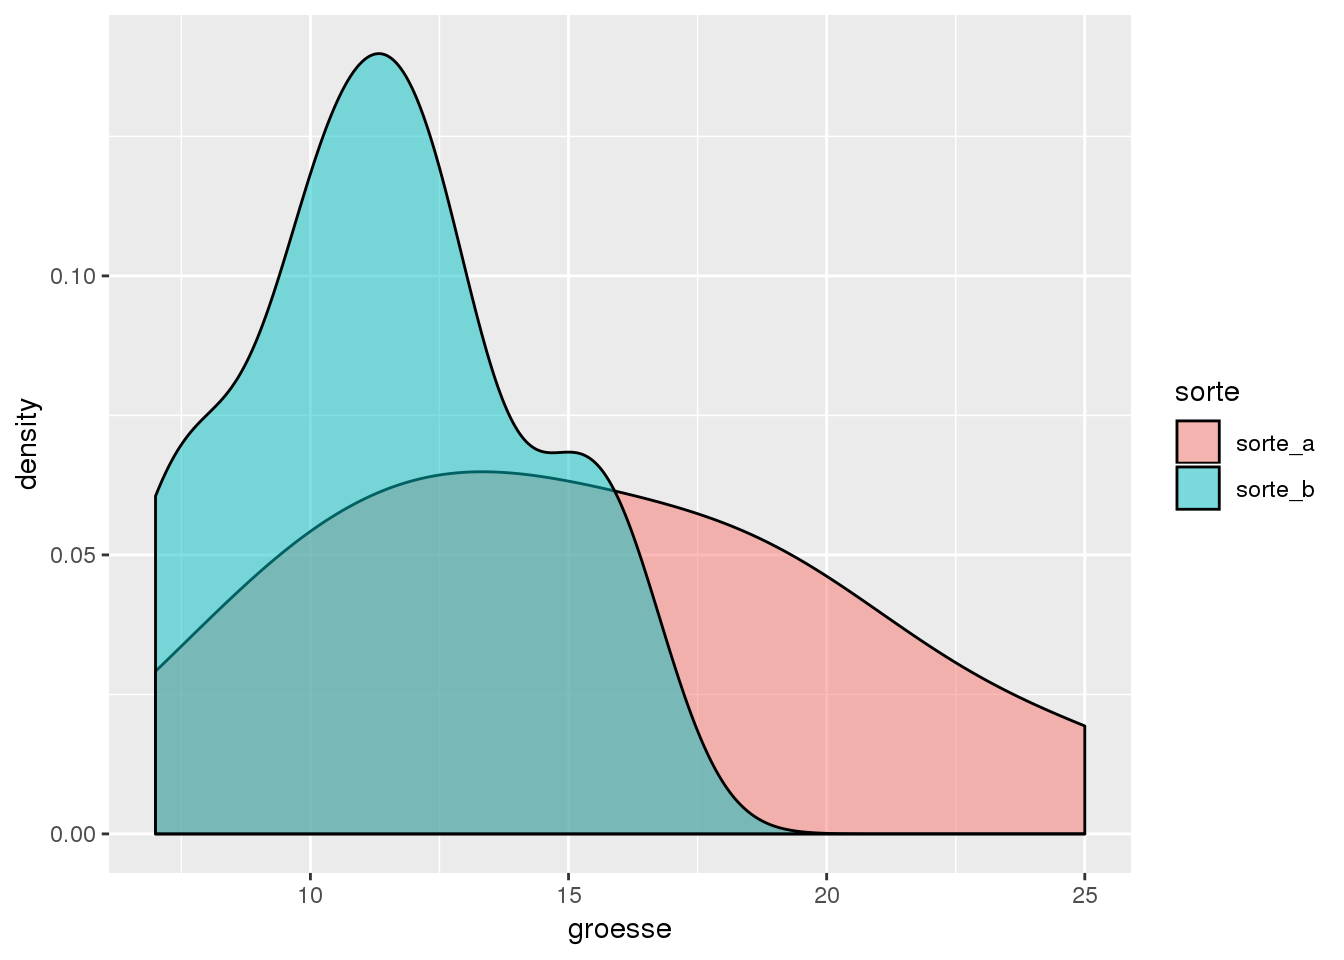
\includegraphics{ResearchMethods_files/figure-latex/unnamed-chunk-12-4.pdf}

\begin{Shaded}
\begin{Highlighting}[]



\NormalTok{tval <-}\StringTok{ }\KeywordTok{length}\NormalTok{(beetles.boot[beetles.boot}\OperatorTok{$}\NormalTok{t }\OperatorTok{>=}\StringTok{ }\KeywordTok{abs}\NormalTok{(beetles.boot}\OperatorTok{$}\NormalTok{t0)])}\OperatorTok{+}\DecValTok{1}

\NormalTok{tval}
\NormalTok{## [1] 50}

\NormalTok{tval}\OperatorTok{/}\NormalTok{(beetles.boot}\OperatorTok{$}\NormalTok{R }\OperatorTok{+}\StringTok{ }\DecValTok{1}\NormalTok{)}
\NormalTok{## [1] 0.009998}
\end{Highlighting}
\end{Shaded}

\subsection{Voraussetzungen parametrischer
Verfahren}\label{voraussetzungen-parametrischer-verfahren}

\subsubsection{F-Test}\label{f-test}

\begin{Shaded}
\begin{Highlighting}[]

\CommentTok{# F-Test}

\KeywordTok{var.test}\NormalTok{(blume}\OperatorTok{$}\NormalTok{sorte_a,blume}\OperatorTok{$}\NormalTok{sorte_b)}
\NormalTok{## }
\NormalTok{##  F test to compare two variances}
\NormalTok{## }
\NormalTok{## data:  blume$sorte_a and blume$sorte_b}
\NormalTok{## F = 3.3715, num df = 9, denom df = 9, p-value = 0.08467}
\NormalTok{## alternative hypothesis: true ratio of variances is not equal to 1}
\NormalTok{## 95 percent confidence interval:}
\NormalTok{##   0.8374446 13.5738284}
\NormalTok{## sample estimates:}
\NormalTok{## ratio of variances }
\NormalTok{##           3.371547}
\KeywordTok{var.test}\NormalTok{(groesse}\OperatorTok{~}\NormalTok{sorte, blume_long)}
\NormalTok{## }
\NormalTok{##  F test to compare two variances}
\NormalTok{## }
\NormalTok{## data:  groesse by sorte}
\NormalTok{## F = 3.3715, num df = 9, denom df = 9, p-value = 0.08467}
\NormalTok{## alternative hypothesis: true ratio of variances is not equal to 1}
\NormalTok{## 95 percent confidence interval:}
\NormalTok{##   0.8374446 13.5738284}
\NormalTok{## sample estimates:}
\NormalTok{## ratio of variances }
\NormalTok{##           3.371547}
\end{Highlighting}
\end{Shaded}

\subsubsection{Levene Test}\label{levene-test}

\begin{Shaded}
\begin{Highlighting}[]

\CommentTok{# Levene Test }

\KeywordTok{library}\NormalTok{(car)}
\KeywordTok{leveneTest}\NormalTok{(blume}\OperatorTok{$}\NormalTok{sorte_a,blume}\OperatorTok{$}\NormalTok{sorte_b,}\DataTypeTok{center=}\NormalTok{mean)}
\NormalTok{## Warning in leveneTest.default(blume$sorte_a, blume$sorte_b, center = mean):}
\NormalTok{## blume$sorte_b coerced to factor.}
\NormalTok{## Warning in anova.lm(lm(resp ~ group)): ANOVA F-tests on an essentially}
\NormalTok{## perfect fit are unreliable}
\NormalTok{## Levene's Test for Homogeneity of Variance (center = mean)}
\NormalTok{##       Df    F value    Pr(>F)    }
\NormalTok{## group  7 3.0148e+30 < 2.2e-16 ***}
\NormalTok{##        2                         }
\NormalTok{## ---}
\NormalTok{## Signif. codes:  0 '***' 0.001 '**' 0.01 '*' 0.05 '.' 0.1 ' ' 1}
\KeywordTok{leveneTest}\NormalTok{(groesse}\OperatorTok{~}\NormalTok{sorte, blume_long)}
\NormalTok{## Warning in leveneTest.default(y = y, group = group, ...): group coerced to}
\NormalTok{## factor.}
\NormalTok{## Levene's Test for Homogeneity of Variance (center = median)}
\NormalTok{##       Df F value  Pr(>F)  }
\NormalTok{## group  1  3.0507 0.09774 .}
\NormalTok{##       18                  }
\NormalTok{## ---}
\NormalTok{## Signif. codes:  0 '***' 0.001 '**' 0.01 '*' 0.05 '.' 0.1 ' ' 1}
\end{Highlighting}
\end{Shaded}

\subsubsection{Visuelle Inspektion /
Transformation}\label{visuelle-inspektion-transformation}

\begin{Shaded}
\begin{Highlighting}[]

\CommentTok{# Visuelle Inspektion}

\NormalTok{sleep <-}\StringTok{ }\NormalTok{msleep }\OperatorTok
\StringTok{  }\KeywordTok{filter}\NormalTok{(vore }\OperatorTok\StringTok{ }\KeywordTok{c}\NormalTok{(}\StringTok{"carni"}\NormalTok{,}\StringTok{"herbi"}\NormalTok{)) }\OperatorTok
\StringTok{  }\NormalTok{dplyr}\OperatorTok{::}\KeywordTok{select}\NormalTok{(name,vore,bodywt)}


\KeywordTok{ggplot}\NormalTok{(sleep, }\KeywordTok{aes}\NormalTok{(vore, bodywt, }\DataTypeTok{group =}\NormalTok{ vore)) }\OperatorTok{+}
\StringTok{  }\KeywordTok{geom_boxplot}\NormalTok{()}
\end{Highlighting}
\end{Shaded}

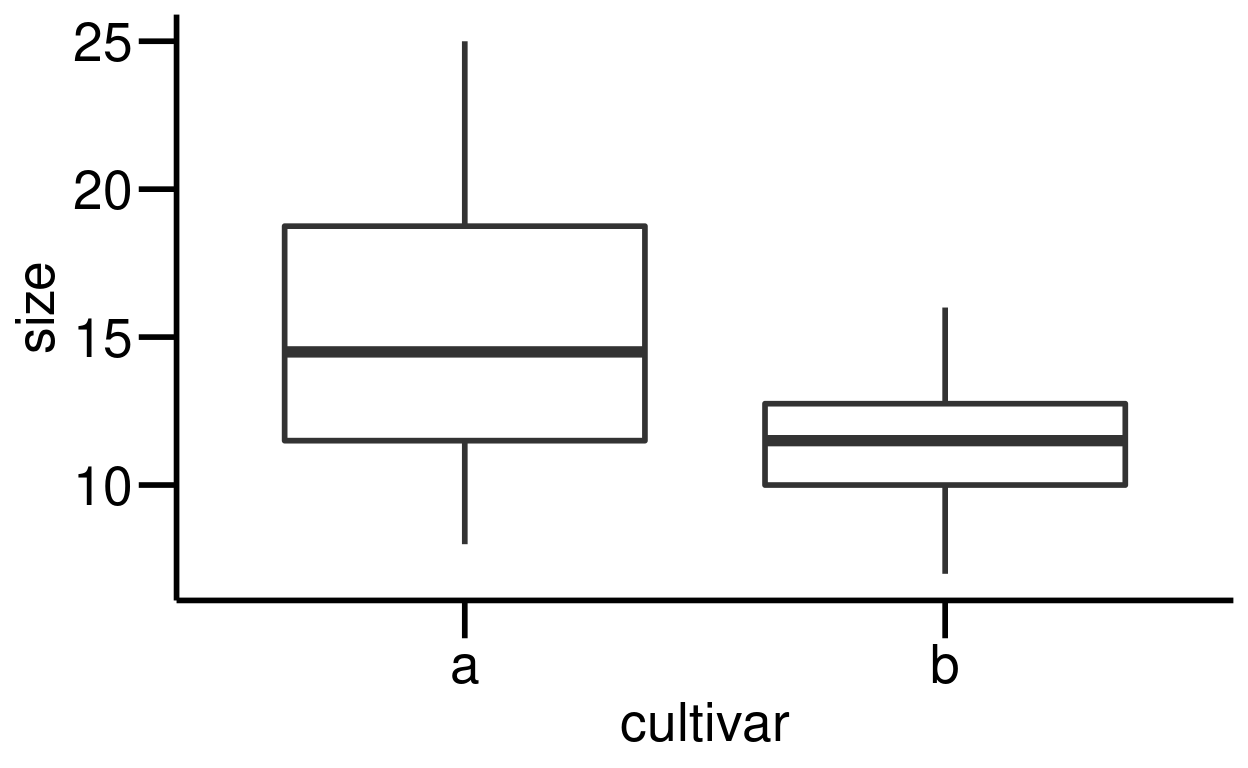
\includegraphics{ResearchMethods_files/figure-latex/unnamed-chunk-15-1.pdf}

\begin{Shaded}
\begin{Highlighting}[]


\NormalTok{sleep <-}\StringTok{ }\NormalTok{sleep }\OperatorTok
\StringTok{  }\KeywordTok{mutate}\NormalTok{(}
    \DataTypeTok{bodywt_log10 =} \KeywordTok{log10}\NormalTok{(bodywt),}
    \DataTypeTok{bodywt_sqrt =} \KeywordTok{sqrt}\NormalTok{(bodywt),}
    \DataTypeTok{bodywt_4throot =}\NormalTok{ bodywt}\OperatorTok{^}\FloatTok{0.25}
\NormalTok{  ) }\OperatorTok
\StringTok{  }\KeywordTok{gather}\NormalTok{(key,val, }\OperatorTok{-}\KeywordTok{c}\NormalTok{(name,vore))}

\NormalTok{sleep}
\NormalTok{## # A tibble: 204 x 4}
\NormalTok{##    name              vore  key        val}
\NormalTok{##    <chr>             <chr> <chr>    <dbl>}
\NormalTok{##  1 Cheetah           carni bodywt  50    }
\NormalTok{##  2 Mountain beaver   herbi bodywt   1.35 }
\NormalTok{##  3 Cow               herbi bodywt 600    }
\NormalTok{##  4 Three-toed sloth  herbi bodywt   3.85 }
\NormalTok{##  5 Northern fur seal carni bodywt  20.5  }
\NormalTok{##  6 Dog               carni bodywt  14    }
\NormalTok{##  7 Roe deer          herbi bodywt  14.8  }
\NormalTok{##  8 Goat              herbi bodywt  33.5  }
\NormalTok{##  9 Guinea pig        herbi bodywt   0.728}
\NormalTok{## 10 Chinchilla        herbi bodywt   0.42 }
\NormalTok{## # ... with 194 more rows}


\KeywordTok{ggplot}\NormalTok{(sleep, }\KeywordTok{aes}\NormalTok{(vore, val, }\DataTypeTok{group =}\NormalTok{ vore)) }\OperatorTok{+}
\StringTok{  }\KeywordTok{geom_boxplot}\NormalTok{() }\OperatorTok{+}
\StringTok{  }\KeywordTok{facet_wrap}\NormalTok{(}\OperatorTok{~}\NormalTok{key, }\DataTypeTok{scales =} \StringTok{"free_y"}\NormalTok{)}
\end{Highlighting}
\end{Shaded}

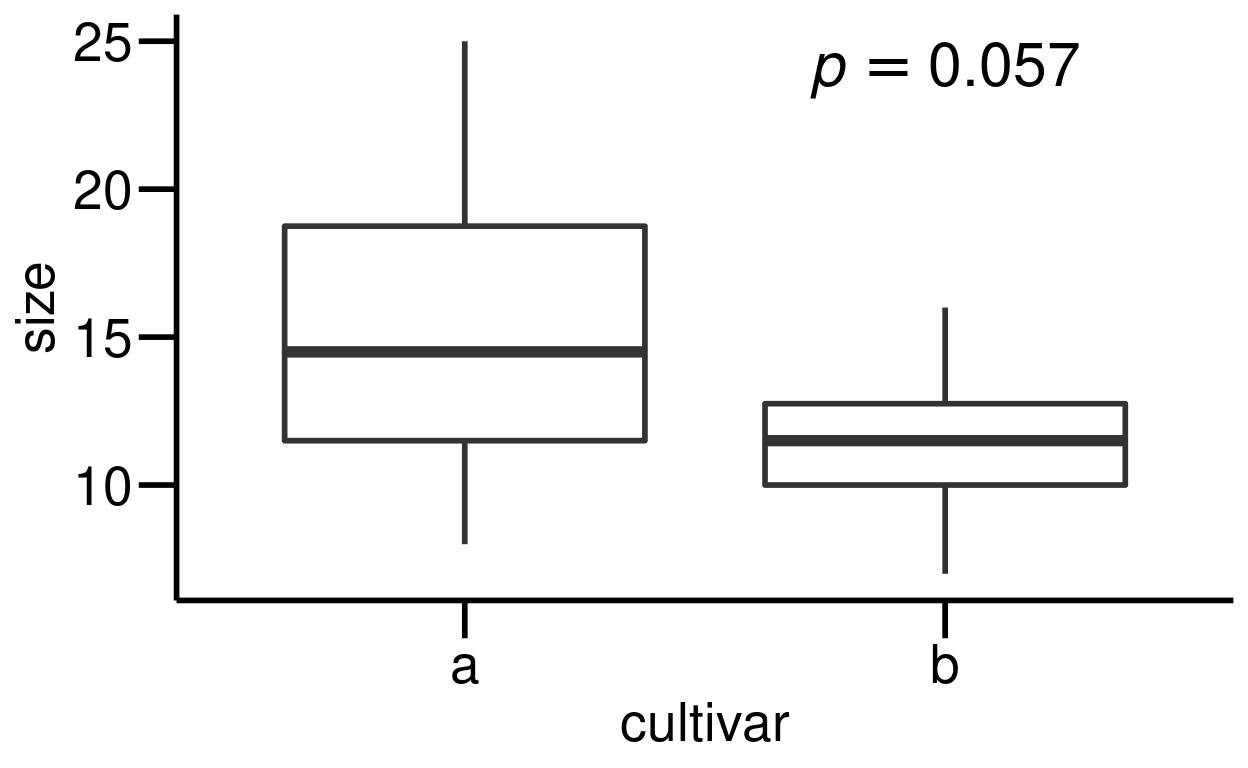
\includegraphics{ResearchMethods_files/figure-latex/unnamed-chunk-15-2.pdf}

\subsection{Einstieg ANOVA}\label{einstieg-anova}

\subsubsection{\texorpdfstring{ANOVA mit
``Blumen''-Daten}{ANOVA mit Blumen-Daten}}\label{anova-mit-blumen-daten}

\begin{Shaded}
\begin{Highlighting}[]

\CommentTok{# ANOVA mit "Blumen"-Daten}

\KeywordTok{ggplot}\NormalTok{(blume_long, }\KeywordTok{aes}\NormalTok{(sorte, groesse)) }\OperatorTok{+}
\StringTok{  }\KeywordTok{geom_boxplot}\NormalTok{()}
\end{Highlighting}
\end{Shaded}

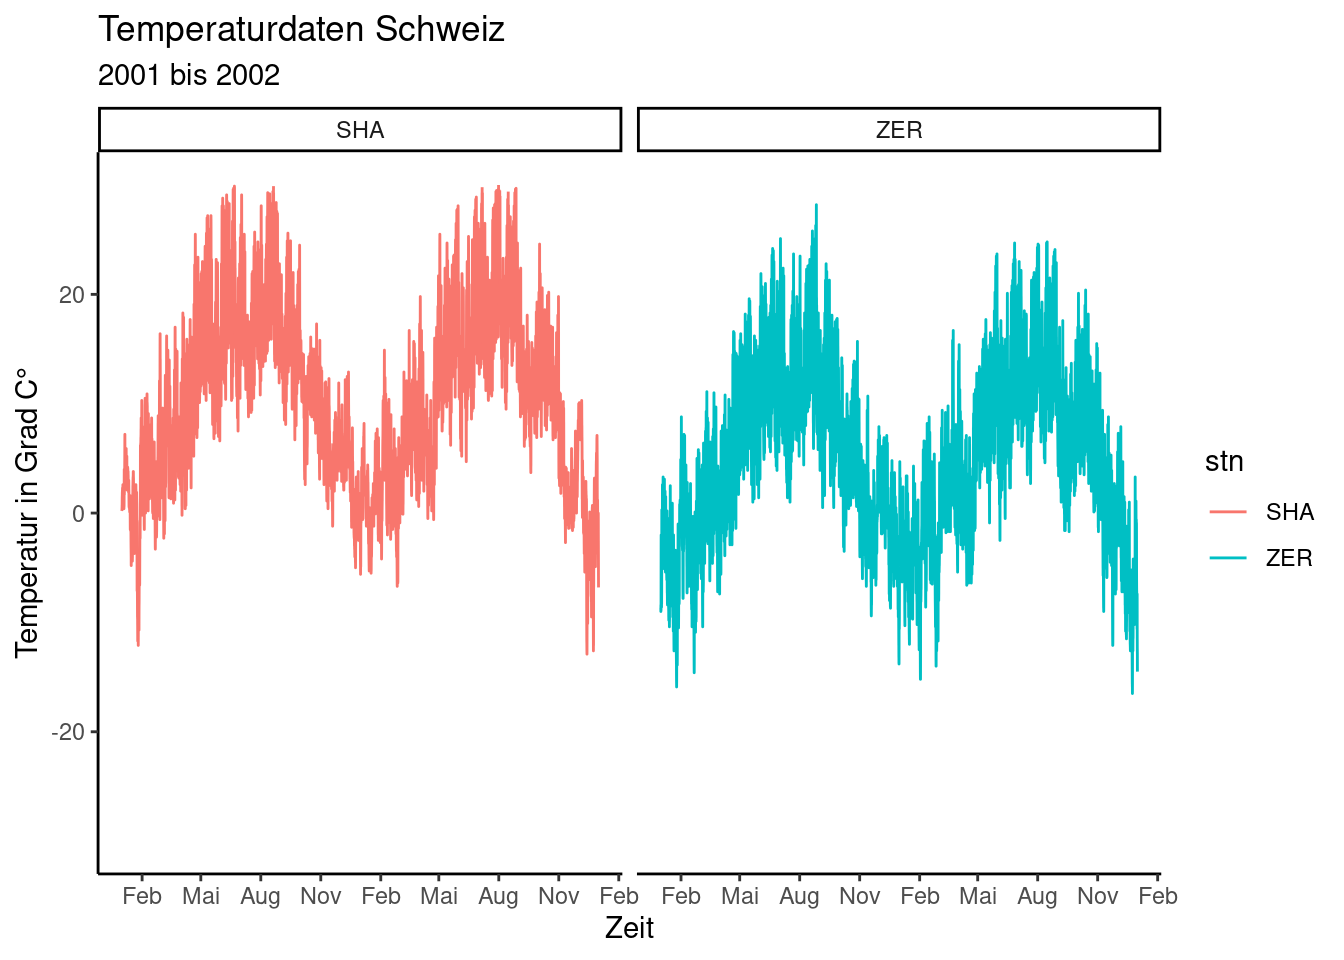
\includegraphics{ResearchMethods_files/figure-latex/unnamed-chunk-16-1.pdf}

\begin{Shaded}
\begin{Highlighting}[]

\KeywordTok{t.test}\NormalTok{(groesse}\OperatorTok{~}\NormalTok{sorte, blume_long, }\DataTypeTok{var.equal=}\NormalTok{T)}
\NormalTok{## }
\NormalTok{##  Two Sample t-test}
\NormalTok{## }
\NormalTok{## data:  groesse by sorte}
\NormalTok{## t = 2.0797, df = 18, p-value = 0.05212}
\NormalTok{## alternative hypothesis: true difference in means is not equal to 0}
\NormalTok{## 95 percent confidence interval:}
\NormalTok{##  -0.03981237  7.83981237}
\NormalTok{## sample estimates:}
\NormalTok{## mean in group sorte_a mean in group sorte_b }
\NormalTok{##                  15.3                  11.4}

\CommentTok{#now as ANOVA}

\KeywordTok{aov}\NormalTok{(groesse}\OperatorTok{~}\NormalTok{sorte,blume_long)}
\NormalTok{## Call:}
\NormalTok{##    aov(formula = groesse ~ sorte, data = blume_long)}
\NormalTok{## }
\NormalTok{## Terms:}
\NormalTok{##                  sorte Residuals}
\NormalTok{## Sum of Squares   76.05    316.50}
\NormalTok{## Deg. of Freedom      1        18}
\NormalTok{## }
\NormalTok{## Residual standard error: 4.193249}
\NormalTok{## Estimated effects may be unbalanced}
\KeywordTok{summary}\NormalTok{(}\KeywordTok{aov}\NormalTok{(groesse}\OperatorTok{~}\NormalTok{sorte,blume_long)) }\CommentTok{#F-value = 4.325}
\NormalTok{##             Df Sum Sq Mean Sq F value Pr(>F)  }
\NormalTok{## sorte        1   76.0   76.05   4.325 0.0521 .}
\NormalTok{## Residuals   18  316.5   17.58                 }
\NormalTok{## ---}
\NormalTok{## Signif. codes:  0 '***' 0.001 '**' 0.01 '*' 0.05 '.' 0.1 ' ' 1}
\KeywordTok{summary.lm}\NormalTok{(}\KeywordTok{aov}\NormalTok{(groesse}\OperatorTok{~}\NormalTok{sorte,blume_long))}
\NormalTok{## }
\NormalTok{## Call:}
\NormalTok{## aov(formula = groesse ~ sorte, data = blume_long)}
\NormalTok{## }
\NormalTok{## Residuals:}
\NormalTok{##    Min     1Q Median     3Q    Max }
\NormalTok{## -7.300 -2.575 -0.350  2.925  9.700 }
\NormalTok{## }
\NormalTok{## Coefficients:}
\NormalTok{##              Estimate Std. Error t value Pr(>|t|)    }
\NormalTok{## (Intercept)    15.300      1.326   11.54 9.47e-10 ***}
\NormalTok{## sortesorte_b   -3.900      1.875   -2.08   0.0521 .  }
\NormalTok{## ---}
\NormalTok{## Signif. codes:  0 '***' 0.001 '**' 0.01 '*' 0.05 '.' 0.1 ' ' 1}
\NormalTok{## }
\NormalTok{## Residual standard error: 4.193 on 18 degrees of freedom}
\NormalTok{## Multiple R-squared:  0.1937, Adjusted R-squared:  0.1489 }
\NormalTok{## F-statistic: 4.325 on 1 and 18 DF,  p-value: 0.05212}

\KeywordTok{lm}\NormalTok{(groesse}\OperatorTok{~}\NormalTok{sorte,blume_long)}
\NormalTok{## }
\NormalTok{## Call:}
\NormalTok{## lm(formula = groesse ~ sorte, data = blume_long)}
\NormalTok{## }
\NormalTok{## Coefficients:}
\NormalTok{##  (Intercept)  sortesorte_b  }
\NormalTok{##         15.3          -3.9}
\KeywordTok{summary}\NormalTok{(}\KeywordTok{lm}\NormalTok{(groesse}\OperatorTok{~}\NormalTok{sorte,blume_long))}
\NormalTok{## }
\NormalTok{## Call:}
\NormalTok{## lm(formula = groesse ~ sorte, data = blume_long)}
\NormalTok{## }
\NormalTok{## Residuals:}
\NormalTok{##    Min     1Q Median     3Q    Max }
\NormalTok{## -7.300 -2.575 -0.350  2.925  9.700 }
\NormalTok{## }
\NormalTok{## Coefficients:}
\NormalTok{##              Estimate Std. Error t value Pr(>|t|)    }
\NormalTok{## (Intercept)    15.300      1.326   11.54 9.47e-10 ***}
\NormalTok{## sortesorte_b   -3.900      1.875   -2.08   0.0521 .  }
\NormalTok{## ---}
\NormalTok{## Signif. codes:  0 '***' 0.001 '**' 0.01 '*' 0.05 '.' 0.1 ' ' 1}
\NormalTok{## }
\NormalTok{## Residual standard error: 4.193 on 18 degrees of freedom}
\NormalTok{## Multiple R-squared:  0.1937, Adjusted R-squared:  0.1489 }
\NormalTok{## F-statistic: 4.325 on 1 and 18 DF,  p-value: 0.05212}

\CommentTok{# Compare the above results of t.test, aov and lm and how the relevant data are displayed}

\CommentTok{# Now check with the F-distribution:}
\CommentTok{# What would have been the critical value for a significant result at p < 0.05?}

\KeywordTok{qf}\NormalTok{(}\FloatTok{0.95}\NormalTok{,}\DecValTok{1}\NormalTok{,}\DecValTok{18}\NormalTok{)}
\NormalTok{## [1] 4.413873}

\CommentTok{# which is the p-value associated with the obtained F-value?}

\DecValTok{1}\OperatorTok{-}\KeywordTok{pf}\NormalTok{(}\FloatTok{4.325}\NormalTok{,}\DecValTok{1}\NormalTok{,}\DecValTok{18}\NormalTok{) }\CommentTok{#probability of obtaining F=4,325 or greater}
\NormalTok{## [1] 0.05212253}
\end{Highlighting}
\end{Shaded}

\begin{Shaded}
\begin{Highlighting}[]
\NormalTok{## Optional für Demo}

\CommentTok{#overall mean and residuals}

\NormalTok{blume_long}\OperatorTok{$}\NormalTok{index <-}\StringTok{ }\DecValTok{1}\OperatorTok{:}\DecValTok{20}

\NormalTok{blume_long <-}\StringTok{ }\NormalTok{blume_long }\OperatorTok
\StringTok{  }\KeywordTok{group_by}\NormalTok{(sorte) }\OperatorTok
\StringTok{  }\KeywordTok{mutate}\NormalTok{(}
    \DataTypeTok{mean =} \KeywordTok{mean}\NormalTok{(groesse)}
\NormalTok{  )}

\KeywordTok{ggplot}\NormalTok{(blume_long, }\KeywordTok{aes}\NormalTok{(index,groesse)) }\OperatorTok{+}
\StringTok{  }\KeywordTok{geom_point}\NormalTok{() }\OperatorTok{+}
\StringTok{  }\KeywordTok{geom_hline}\NormalTok{(}\KeywordTok{aes}\NormalTok{(}\DataTypeTok{yintercept =}  \KeywordTok{mean}\NormalTok{(groesse))) }\OperatorTok{+}
\StringTok{  }\KeywordTok{geom_segment}\NormalTok{(}\KeywordTok{aes}\NormalTok{(}\DataTypeTok{x =}\NormalTok{ index,}\DataTypeTok{y =}\NormalTok{ groesse,}\DataTypeTok{xend =}\NormalTok{ index,}\DataTypeTok{yend =} \KeywordTok{mean}\NormalTok{(groesse))) }\OperatorTok{+}
\StringTok{  }\KeywordTok{labs}\NormalTok{(}\DataTypeTok{x =} \StringTok{"Order"}\NormalTok{,}\DataTypeTok{y =} \KeywordTok{expression}\NormalTok{(Size}\OperatorTok{~}\NormalTok{(cm}\OperatorTok{^}\DecValTok{2}\NormalTok{)))}
\end{Highlighting}
\end{Shaded}

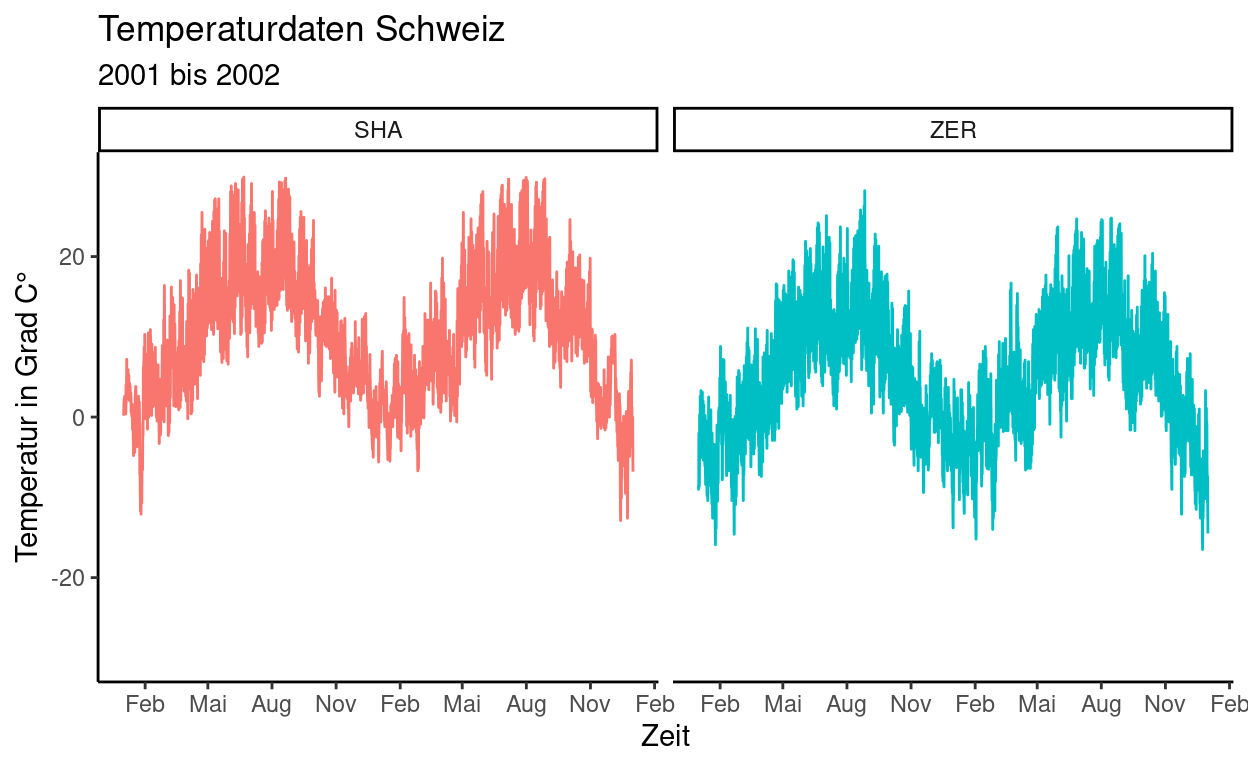
\includegraphics{ResearchMethods_files/figure-latex/unnamed-chunk-17-1.pdf}

\begin{Shaded}
\begin{Highlighting}[]

\CommentTok{#group means and residuals}

\KeywordTok{ggplot}\NormalTok{(blume_long, }\KeywordTok{aes}\NormalTok{(index,groesse, }\DataTypeTok{colour =}\NormalTok{ sorte)) }\OperatorTok{+}
\StringTok{  }\KeywordTok{geom_point}\NormalTok{() }\OperatorTok{+}
\StringTok{  }\KeywordTok{geom_hline}\NormalTok{(}\KeywordTok{aes}\NormalTok{(}\DataTypeTok{yintercept =}\NormalTok{ mean)) }\OperatorTok{+}
\StringTok{  }\KeywordTok{geom_segment}\NormalTok{(}\KeywordTok{aes}\NormalTok{(}\DataTypeTok{x =}\NormalTok{ index,}\DataTypeTok{y =}\NormalTok{ groesse,}\DataTypeTok{xend =}\NormalTok{ index,}\DataTypeTok{yend =}\NormalTok{ mean)) }\OperatorTok{+}
\StringTok{  }\KeywordTok{labs}\NormalTok{(}\DataTypeTok{x =} \StringTok{"Order"}\NormalTok{,}\DataTypeTok{y =} \KeywordTok{expression}\NormalTok{(Size}\OperatorTok{~}\NormalTok{(cm}\OperatorTok{^}\DecValTok{2}\NormalTok{))) }\OperatorTok{+}
\StringTok{  }\KeywordTok{facet_grid}\NormalTok{(}\OperatorTok{~}\NormalTok{sorte)}
\end{Highlighting}
\end{Shaded}

\includegraphics{ResearchMethods_files/figure-latex/unnamed-chunk-17-2.pdf}

\begin{Shaded}
\begin{Highlighting}[]



\KeywordTok{library}\NormalTok{(ggfortify)}

\KeywordTok{autoplot}\NormalTok{(}\KeywordTok{aov}\NormalTok{(groesse}\OperatorTok{~}\NormalTok{sorte, blume_long))}
\end{Highlighting}
\end{Shaded}

\includegraphics{ResearchMethods_files/figure-latex/unnamed-chunk-17-3.pdf}

\subsubsection{ANOVA mit Gewässerdaten}\label{anova-mit-gewasserdaten}

Aus Logan (\protect\hyperlink{ref-logan2010}{2010} S. 265): Script an
Tools/Packages des Moduls Research Methods angepasst

Medley and Clements (1998) investigated the impact of zinc contamination
(and other heavy metals) on the diversity of diatom species in the USA
Rocky Mountains (from Box 8.1 of Quinn and Keough (2002)). The diversity
of diatoms (number of species) and degree of zinc contamination
(categorized as either of high, medium, low or natural background level)
were recorded from between four and six sampling stations within each of
six streams known to be polluted. These data were used to test the null
hypothesis that there were no differences the diversity of diatoms
between different zinc levels
(\[H_0 = \mu_M = \mu_L = \mu_V = \mu; \alpha_i = 0\])

The linear effects model would be:

\[\gamma_{ij} = \mu + \alpha_i + \epsilon_{ij}\]
\[\text{diatom species diversity} = \text{overal mean} + \text{effect of zinc level} + \text{error}\]

\paragraph{Step 1}\label{step-1}

Import the Medley and Clements (1998) data set
\href{13_Statistik1/data/medley.csv}{medley.csv}

\begin{Shaded}
\begin{Highlighting}[]

\CommentTok{# impact of zinc contamination (and other heavy metals) on the diversity of diatom species in the USA Rocky Mountains}

\NormalTok{medley <-}\StringTok{ }\KeywordTok{read_delim}\NormalTok{(}\StringTok{"13_Statistik1/data/medley.csv"}\NormalTok{, }\StringTok{","}\NormalTok{)}
\NormalTok{## Parsed with column specification:}
\NormalTok{## cols(}
\NormalTok{##   STREAM = col_character(),}
\NormalTok{##   ZINC = col_character(),}
\NormalTok{##   DIVERSITY = col_double()}
\NormalTok{## )}
\end{Highlighting}
\end{Shaded}

\paragraph{Step 2}\label{step-2}

Reorganize the levels of the categorical factor into a more logical
order

\begin{Shaded}
\begin{Highlighting}[]

\CommentTok{# Reorganize the levels of the categorical factor into a more logical order}

\NormalTok{medley}\OperatorTok{$}\NormalTok{ZINC <-}\StringTok{ }\KeywordTok{factor}\NormalTok{(medley}\OperatorTok{$}\NormalTok{ZINC, }\DataTypeTok{levels=}\KeywordTok{c}\NormalTok{(}\StringTok{"BACK"}\NormalTok{, }\StringTok{"LOW"}\NormalTok{, }\StringTok{"MED"}\NormalTok{,}\StringTok{"HIGH"}\NormalTok{), }\DataTypeTok{ordered=}\NormalTok{T)}
\end{Highlighting}
\end{Shaded}

\paragraph{Step 3}\label{step-3}

Assess normality/homogeneity of variance using boxplot of species
diversity against zinc group

\begin{Shaded}
\begin{Highlighting}[]

\CommentTok{# Assess normality/homogeneity of variance using boxplot of species diversity against zinc group}

\KeywordTok{ggplot}\NormalTok{(medley, }\KeywordTok{aes}\NormalTok{(ZINC, DIVERSITY)) }\OperatorTok{+}
\StringTok{  }\KeywordTok{geom_boxplot}\NormalTok{()}
\end{Highlighting}
\end{Shaded}

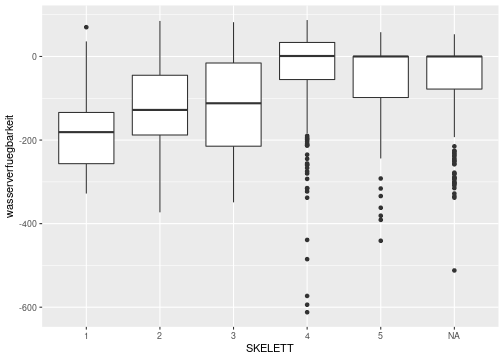
\includegraphics{ResearchMethods_files/figure-latex/unnamed-chunk-20-1.pdf}

\paragraph{Step 4}\label{step-4}

Assess homogeneity of variance assumption with a table and/or plot of
mean vs variance

\begin{Shaded}
\begin{Highlighting}[]

\CommentTok{# Assess homogeneity of variance assumption with a table and/or plot of mean vs variance}

\NormalTok{medley_sry <-}\StringTok{ }\NormalTok{medley }\OperatorTok
\StringTok{  }\KeywordTok{group_by}\NormalTok{(ZINC) }\OperatorTok
\StringTok{  }\KeywordTok{summarise}\NormalTok{(}
    \DataTypeTok{mean =} \KeywordTok{mean}\NormalTok{(DIVERSITY),}
    \DataTypeTok{var =} \KeywordTok{var}\NormalTok{(DIVERSITY),}
    \DataTypeTok{sd =} \KeywordTok{sd}\NormalTok{(DIVERSITY)}
\NormalTok{  )}

\KeywordTok{ggplot}\NormalTok{(medley_sry, }\KeywordTok{aes}\NormalTok{(mean,var)) }\OperatorTok{+}
\StringTok{  }\KeywordTok{geom_point}\NormalTok{()}
\end{Highlighting}
\end{Shaded}

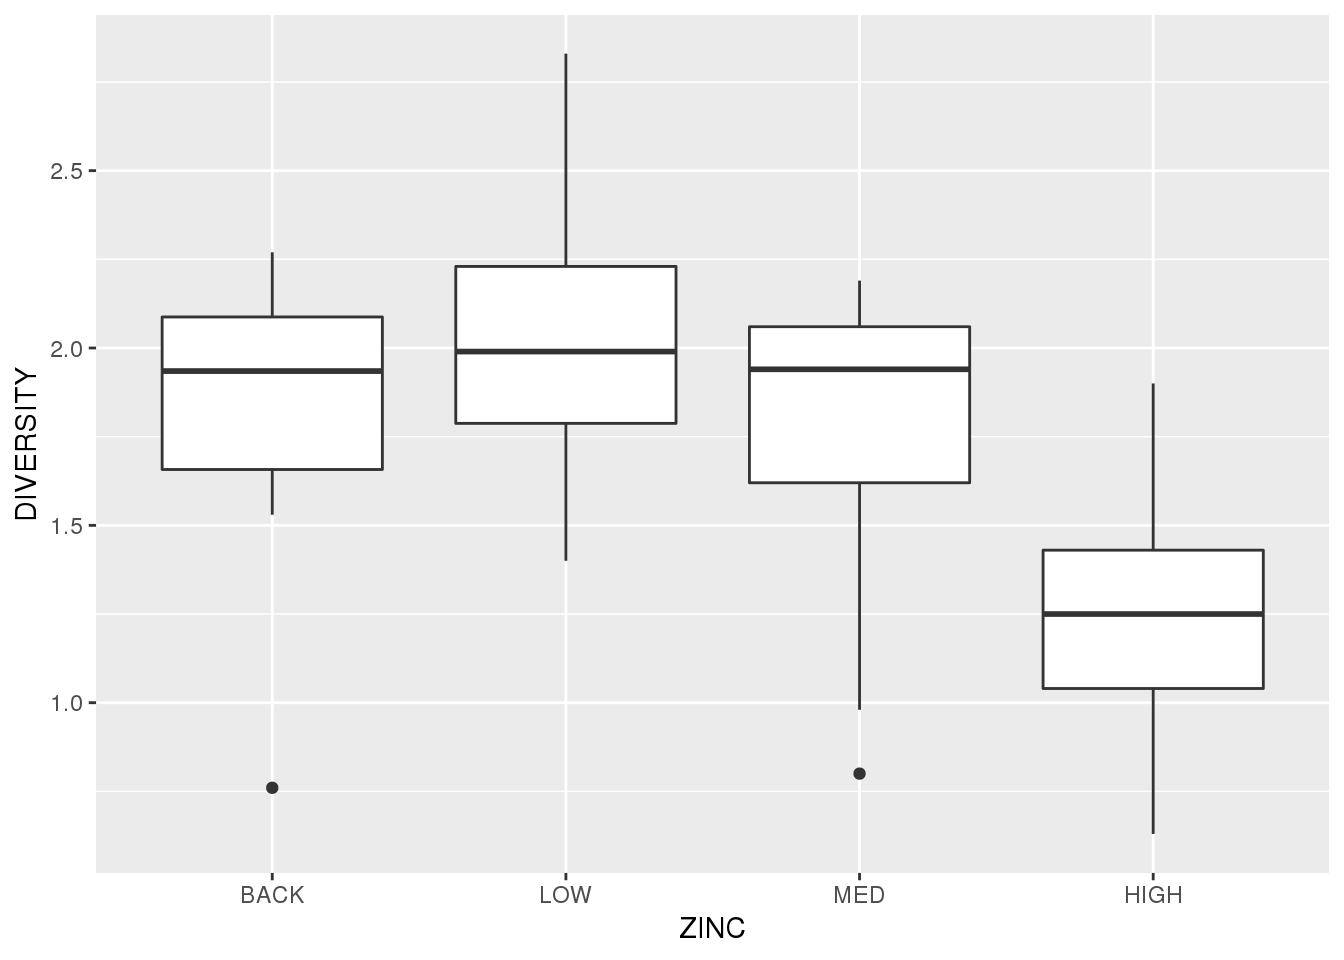
\includegraphics{ResearchMethods_files/figure-latex/unnamed-chunk-21-1.pdf}

\subsection{Libraries}\label{libraries}

Dieses Kapitel verwendet folgende Libraries: Canty and Ripley
(\protect\hyperlink{ref-R-boot}{2017}), Horikoshi and Tang
(\protect\hyperlink{ref-R-ggfortify}{2017}), ({\textbf{???}}), Wickham
(\protect\hyperlink{ref-R-stringr}{2017}\protect\hyperlink{ref-R-stringr}{a}),
Wickham et al. (\protect\hyperlink{ref-R-dplyr}{2017}), Henry and
Wickham (\protect\hyperlink{ref-R-purrr}{2017}), Wickham, Hester, and
Francois (\protect\hyperlink{ref-R-readr}{2017}), Wickham and Henry
(\protect\hyperlink{ref-R-tidyr}{2017}), Müller and Wickham
(\protect\hyperlink{ref-R-tibble}{2017}), Wickham and Chang
(\protect\hyperlink{ref-R-ggplot2}{2016}), Wickham
(\protect\hyperlink{ref-R-tidyverse}{2017}\protect\hyperlink{ref-R-tidyverse}{b}),
Fox and Weisberg (\protect\hyperlink{ref-R-car}{2017}), ({\textbf{???}})

\section{Beschreibung Forschungsprojekt NOVANIMAL
(NFP69)}\label{beschreibung-forschungsprojekt-novanimal-nfp69}

\subsection{Innovationen für zukunftsorientierte Ernährung und
Lebensmittelproduktion}\label{innovationen-fur-zukunftsorientierte-ernahrung-und-lebensmittelproduktion}

Die Menschen essen weltweit immer mehr Fleisch- und Milchprodukte
(FAOSTAT
\protect\hyperlink{ref-food_and_agriculture_organization_of_the_united_nations_statistics_faostat_commodity_2017}{2017}).
Aus ökologischen und gesundheitlichen Gründen ist diese Entwicklung
problematisch, denn für die Produktion von tierischen Nahrungsmitteln
braucht es mehr Boden, Wasser und Energie als bei der Produktion
pflanzlicher Nahrungsmittel und auch die Umweltbelastungen sind höher
als bei der pflanzlichen Produktion (Westhoek et al.
\protect\hyperlink{ref-westhoek_food_2014}{2014}). Zudem sind tierische
Nahrungsmittel energiedicht und können zu Übergewicht und zu
entsprechenden Folgeerkrankungen beitragen. Des Weiteren stehen manche
Fleischsorten im Verdacht, das Risiko für Krebs- und
Herzkreislaufkrankheiten zu erhöhen (Tilman and Clark
\protect\hyperlink{ref-tilman_global_2014}{2014}).

Der Pro-Kopf-Konsum an Fleisch und Milch ist in der Schweiz deutlich
höher als im globalen Durchschnitt. Aus ökologischen und
gesundheitlichen Gründen ist auch in der Schweiz ein moderater Konsum
wünschenswert (Johnston, Fanzo, and Cogill
\protect\hyperlink{ref-johnston_understanding_2014}{2014}; Macdiarmid
\protect\hyperlink{ref-macdiarmid_is_2013}{2013}; Marlow et al.
\protect\hyperlink{ref-marlow_diet_2009}{2009}; Tukker et al.
\protect\hyperlink{ref-tukker_environmental_2011}{2011}). Was aber
heisst das für eine liberale Gesellschaft (Kamm et al.
\protect\hyperlink{ref-kamm_ernahrung_2015}{2015})? Was braucht es,
damit Menschen freiwillig weniger tierische Produkte konsumieren?

Ein interessanter Ansatzpunkt ist die Ausser-Haus-Verpflegung. Gemäss
der ersten, in den Jahren 2014/2015 durchgeführten nationalen
Ernährungserhebung menuCH, essen 70\% der Bevölkerung zwischen 18 und 75
Jahren am Mittag auswärts (Bochud et al.
\protect\hyperlink{ref-bochud_anthropometric_2017}{2017}). Daher rückt
die Gastronomie als zentraler Akteur einer innovativen und nachhaltigen
Ernährungswirtschaft ins Blickfeld. Welche Innovationen in der
Gastronomie könnten dazu beitragen, den Pro-Kopf-Verbrauch an tierischen
Nahrungsmitteln zu senken?

Der Fokus liegt in diesem Teilprojekt auf der Schweizer
Gemeinschaftsgastronomie (Forschungsgruppe „Good Pracitice --
Gemeinschaftsgastronomie``
\protect\hyperlink{ref-forschungsgruppe_good_pracitice__gemeinschaftsgastronomie_schweizer_2015}{2015}).
Forschungsleitend ist die Frage, wie die Gäste dazu bewogen werden
können, häufiger ressourcenschonende vegetarische oder ausschliesslich
pflanzliche Gerichte zu wählen.

Zusammen mit den Praxispartnern, einem Catering-Unternehmen und dem
Facility Management einer Hochschule, wurde ein Experiment vorbereitet,
das als Pilotversuch in zwei Hochschulmensen durchgeführt wird. Konkret
wird untersucht, wie die Gäste auf ein verändertes Menü-Angebot mit
einem höheren Anteil an ressourcenschonenden vegetarischen oder rein
pflanzlichen Gerichte reagieren. Eine besondere Herausforderung ist,
dieses erhöhte Angebot in vergleichbarer Qualität wie die der
fleischhaltigen Gerichte anzubieten. Das Küchenteam, das die Gerichte
zubereitet, muss dazu selber innovativ und kreativ sein bzw. bereit
sein, Neues auszuprobieren(Edwards
\protect\hyperlink{ref-edwards_foodservice_2013}{2013}).

Das Experiment findet im Herbstsemester 2017 während 12 Wochen statt und
besteht aus zwei Mensazyklen à 6 Wochen. Über den gesamten
Untersuchungszeitraum werden insgesamt 90 verschiedene Gerichte
angeboten. Das Referenzangebot besteht aus zwei fleisch- oder
fischhaltigen Menüs und einem vegetarischen Angebot. Das veränderte
Menü-(Interventions)-Angebot kehrt das Verhältnis um und beinhaltet ein
ausschliesslich pflanzliches, ein vegetarisches und ein fleisch- oder
fischhaltiges Gericht. Referenz- und Interventionsangebot wechseln
wöchentlich ab. In der Referenz- und in der Basisperiode können die
Gäste jeweils auf ein Buffetangebot ausweichen, indem sie ihre Mahlzeit
aus warmen und kalten Komponenten selber zusammenstellen können. Die
Gerichte werden über drei vorgegebene Menülinien (Favorite, Kitchen,
World) randomisiert angeboten.

Die Abbildung zeigt das Versuchsdesign der ersten 6 Experimentalwochen
(Kalenderwoche 40 bis 45).
\includegraphics{design_experiment_ohne datum_180426_03egel.png}

Mehr Informationen über das Forschungsprojekt NOVANIMAL findet ihr auf
dieser \href{https://www.novanimal.ch}{Webpage}

\hypertarget{refs}{}
\hypertarget{ref-bochud_anthropometric_2017}{}
Bochud, Murielle, Angéline Chatelan, Juan-Manuel Blanco, and Sigrid
Beer-Borst. 2017. ``Anthropometric Characteristics and Indicators of
Eating and Physical Activity Behaviors in the Swiss Adult Population.''
\url{https://www.blv.admin.ch/dam/blv/de/dokumente/lebensmittel-und-ernaehrung/ernaehrung/menuch-bericht.pdf.download.pdf/menuch-bericht.pdf}.

\hypertarget{ref-R-boot}{}
Canty, Angelo, and Brian Ripley. 2017. \emph{Boot: Bootstrap Functions
(Originally by Angelo Canty for S)}.
\url{https://CRAN.R-project.org/package=boot}.

\hypertarget{ref-edwards_foodservice_2013}{}
Edwards, John S.A. 2013. ``The Foodservice Industry: Eating Out Is More
Than Just a Meal.'' \emph{Food Quality and Preference} 27 (2): 223--29.
doi:\href{https://doi.org/10.1016/j.foodqual.2012.02.003}{10.1016/j.foodqual.2012.02.003}.

\hypertarget{ref-food_and_agriculture_organization_of_the_united_nations_statistics_faostat_commodity_2017}{}
FAOSTAT. 2017. ``Commodity Balances - Livestock and Fish Primary
Equivalent.'' \url{http://www.fao.org/faostat/en/\#data/BL}.

\hypertarget{ref-forschungsgruppe_good_pracitice__gemeinschaftsgastronomie_schweizer_2015}{}
Forschungsgruppe „Good Pracitice -- Gemeinschaftsgastronomie``, ed.
2015. \emph{Schweizer Qualitätsstandards Für Eine Gesundheitsfördernde
Gemeinschaftsgastronomie.} 2nd ed. Bern: Berner Fachhochschule,
Fachbereich Gesundheit.

\hypertarget{ref-R-car}{}
Fox, John, and Sanford Weisberg. 2017. \emph{Car: Companion to Applied
Regression}. \url{https://CRAN.R-project.org/package=car}.

\hypertarget{ref-R-purrr}{}
Henry, Lionel, and Hadley Wickham. 2017. \emph{Purrr: Functional
Programming Tools}. \url{https://CRAN.R-project.org/package=purrr}.

\hypertarget{ref-R-ggfortify}{}
Horikoshi, Masaaki, and Yuan Tang. 2017. \emph{Ggfortify: Data
Visualization Tools for Statistical Analysis Results}.
\url{https://CRAN.R-project.org/package=ggfortify}.

\hypertarget{ref-johnston_understanding_2014}{}
Johnston, J. L., J. C. Fanzo, and B. Cogill. 2014. ``Understanding
Sustainable Diets: A Descriptive Analysis of the Determinants and
Processes That Influence Diets and Their Impact on Health, Food
Security, and Environmental Sustainability.'' \emph{Advances in
Nutrition: An International Review Journal} 5 (4): 418--29.
doi:\href{https://doi.org/10.3945/an.113.005553}{10.3945/an.113.005553}.

\hypertarget{ref-kamm_ernahrung_2015}{}
Kamm, A., G. Hildesheimer, E. Bernold, D. Eichhorn, and Bundesamt für
Umwelt (BAFU). 2015. ``Ernährung \& Nachhaltigkeit in Der Schweiz: Eine
Verhaltensökonomische Studie.'' FehrAdvice \& Partners AG.

\hypertarget{ref-logan2010}{}
Logan, Murray. 2010. \emph{Biostatistical Design and Analysis Using R :
A Practical Guide}. Wiley-Blackwell.
\url{http://onlinelibrary.wiley.com/book/10.1002/9781444319620}.

\hypertarget{ref-macdiarmid_is_2013}{}
Macdiarmid, Jennie I. 2013. ``Is a Healthy Diet an Environmentally
Sustainable Diet?'' \emph{Proceedings of the Nutrition Society} 72 (1):
13--20. \url{http://journals.cambridge.org/article_S0029665112002893}.

\hypertarget{ref-marlow_diet_2009}{}
Marlow, Harold J., William K. Hayes, Samuel Soret, Ronald L. Carter,
Ernest R. Schwab, and Joan Sabate. 2009. ``Diet and the Environment:
Does What You Eat Matter?'' \emph{The American Journal of Clinical
Nutrition} 89 (5): 1699S--1703S.
\url{http://ajcn.nutrition.org/content/89/5/1699S.short}.

\hypertarget{ref-R-tibble}{}
Müller, Kirill, and Hadley Wickham. 2017. \emph{Tibble: Simple Data
Frames}. \url{https://CRAN.R-project.org/package=tibble}.

\hypertarget{ref-tilman_global_2014}{}
Tilman, David, and Michael Clark. 2014. ``Global Diets Link
Environmental Sustainability and Human Health.'' \emph{Nature} 515
(7528): 518--22.
doi:\href{https://doi.org/10.1038/nature13959}{10.1038/nature13959}.

\hypertarget{ref-tukker_environmental_2011}{}
Tukker, Arnold, R. Alexandra Goldbohm, Arjan de Koning, Marieke
Verheijden, René Kleijn, Oliver Wolf, Ignacio Pérez-Domínguez, and Jose
M. Rueda-Cantuche. 2011. ``Environmental Impacts of Changes to Healthier
Diets in Europe.'' \emph{Ecological Economics} 70 (10): 1776--88.
doi:\href{https://doi.org/10.1016/j.ecolecon.2011.05.001}{10.1016/j.ecolecon.2011.05.001}.

\hypertarget{ref-westhoek_food_2014}{}
Westhoek, Henk, Jan Peter Lesschen, Trudy Rood, Susanne Wagner,
Alessandra De Marco, Donal Murphy-Bokern, Adrian Leip, Hans van
Grinsven, Mark A. Sutton, and Oene Oenema. 2014. ``Food Choices, Health
and Environment: Effects of Cutting Europe's Meat and Dairy Intake.''
\emph{Global Environmental Change} 26 (May): 196--205.
doi:\href{https://doi.org/10.1016/j.gloenvcha.2014.02.004}{10.1016/j.gloenvcha.2014.02.004}.

\hypertarget{ref-R-stringr}{}
Wickham, Hadley. 2017a. \emph{Stringr: Simple, Consistent Wrappers for
Common String Operations}.
\url{https://CRAN.R-project.org/package=stringr}.

\hypertarget{ref-R-tidyverse}{}
---------. 2017b. \emph{Tidyverse: Easily Install and Load 'Tidyverse'
Packages}. \url{https://CRAN.R-project.org/package=tidyverse}.

\hypertarget{ref-R-ggplot2}{}
Wickham, Hadley, and Winston Chang. 2016. \emph{Ggplot2: Create Elegant
Data Visualisations Using the Grammar of Graphics}.
\url{https://CRAN.R-project.org/package=ggplot2}.

\hypertarget{ref-R-tidyr}{}
Wickham, Hadley, and Lionel Henry. 2017. \emph{Tidyr: Easily Tidy Data
with 'Spread()' and 'Gather()' Functions}.
\url{https://CRAN.R-project.org/package=tidyr}.

\hypertarget{ref-R-dplyr}{}
Wickham, Hadley, Romain Francois, Lionel Henry, and Kirill Müller. 2017.
\emph{Dplyr: A Grammar of Data Manipulation}.
\url{https://CRAN.R-project.org/package=dplyr}.

\hypertarget{ref-R-readr}{}
Wickham, Hadley, Jim Hester, and Romain Francois. 2017. \emph{Readr:
Read Rectangular Text Data}.
\url{https://CRAN.R-project.org/package=readr}.


\end{document}
